\documentclass[14pt,oneside]{extarticle}

\usepackage{amsmath}
\usepackage{unicode-math}
\renewcommand{\familydefault}{\rmdefault}
\usepackage{mathtext}
\usepackage{geometry}
\geometry{verbose,lmargin=25mm,rmargin=15mm,tmargin=15mm,bmargin=20mm}
\setcounter{secnumdepth}{3}
\setcounter{tocdepth}{3}
\usepackage{setspace}
\setstretch{1.5}

% Картинки (можно встявлять даже pdf)
\usepackage{graphicx}

% Таблицы
\usepackage{tabularx}
% \setlength{\extrarowheight}{0.3cm}
\renewcommand{\arraystretch}{1.5}
\renewcommand{\tabularxcolumn}[1]{>{\centering\arraybackslash\small}m{#1}}
\newcolumntype{B}{>{\bfseries\small}c}
\newcolumntype{R}{>{\small}c}
%% Because html converters don't know tabularnewline
\providecommand{\tabularnewline}{\\}

\makeatletter
%%%%%%%%%%%%%%%%%%%%%%%%%%%%%% Textclass specific LaTeX commands.
\numberwithin{figure}{section}
\numberwithin{table}{section}
\numberwithin{equation}{section}
\makeatother

% Абзацный отступ = 1.25см
\usepackage{indentfirst}
\setlength\parindent{12.5mm}

% Пакет для содержания
\usepackage{tocloft}

% Команда для специальных разделов (введение, обзор литературы, etc)
% Не нумеруются в содержании, по уровню вложенности: 
\newcommand{\specialsection}[1]{
    \phantomsection
    \bigskip\smallskip\hspace{-13.8mm}
    \normalfont\fontsize{18}{18}\textbf{#1}
    \par\bigskip\normalfont\normalsize
    \addcontentsline{toc}{section}{#1}
}

% Размеры заголовков разделов и подразделов
\usepackage{titlesec}
% Раздел: 18pt, добавляем слово "Глава"
\titleformat{\section}
{\fontsize{18}{18}\bfseries}{
\hspace{-1.5mm}Глава \thesection. \hskip-1em}{1em}{}
% Подраздел: 16pt
\titleformat{\subsection}
{\fontsize{16}{16}\bfseries}{\hspace{-0.2mm}\thesubsection}{1em}{}

% Содержание
% Выравнивание заголовка по центру (да, да, с отступом слева)
% т.к. окружение center и \centering не работают
\renewcommand{\cfttoctitlefont}{\hspace{0.35\textwidth} \bfseries\Large}
% \renewcommand{\cftbeforetoctitleskip}{3em}
% Слово "Глава" в содержании
\renewcommand{\cftsecpresnum}{Глава\space}
\newlength\mylength
\settowidth\mylength{\cftsecpresnum}
\addtolength\cftsecnumwidth{1.5\mylength}
% Строки с точками
\renewcommand{\cftsecleader}{\cftdotfill{\cftdotsep}}
% Точки после цифр в в содержании
\renewcommand{\cftsecaftersnum}{.}
\renewcommand{\cftsubsecaftersnum}{.}
% Подровнять subsection под точку главы
% (если глав будет больше десяти, будет чуть хуже)
\setlength{\cftsubsecindent}{2em}
% Интервал глав
\setlength{\cftbeforesecskip}{3pt}

\renewcommand{\cftsecpagefont}{\normalfont}

\usepackage[russian]{babel}
\usepackage{fontspec}
\setmainfont{Times New Roman}
\setmathfont{TeX Gyre Termes Math}
\usepackage{csquotes}

% Пакет, реализующий гиперссылки. Никакого расскрашивания
\usepackage[colorlinks=false,unicode=true,hidelinks]{hyperref}

\newcommand{\ITEM}{\vspace{-0.2cm}\item}
\newcommand{\MList}[1]{\par\begin{itemize}#1\end{itemize}}
\newcommand{\NList}[1]{\par\begin{enumerate}#1\end{enumerate}}

% Шрифт подписи (caption) = 12pt
% (Повезло, что small как раз равен 12pt)
\usepackage[font=small,labelfont=bf]{caption}

% Пакет, который позволяет собирать один документ TeX из нескольких
\usepackage{import}

%Библиография
\usepackage[
    backend=biber,
    %citestyle = alphabetic, 
    %bibstyle = ieee-alphabetic,  
    %sortlocale=en_US,
    sorting=none,
    backref=true,
    hyperref=true,
    style=numeric,%style=alphabetic,
    defernumbers=true,
    isbn=false,
    autolang=none,
    %eid=true,
    doi=false,
    %series=true,
    eprint=false,
    bibencoding = utf8
]{biblatex} %Imports biblatex package

\renewbibmacro{volume+number+eid}{%
    \printfield{volume}%
    \setunit{\addcomma\space}%
    \printfield{number}%
    \printfield{eid}}

\renewbibmacro{in:}{\space}

\DeclareFieldFormat[article]{volume}{{том}\space#1}
\DeclareFieldFormat[article]{number}{{номер}\space#1\addcomma}

\DefineBibliographyStrings{russian}{%
    phdthesis = {диссертация}%
}

\addbibresource{literature.bib} %Import the bibliography file

% Подсветка кода (все стили в файле)
\usepackage{color}
\usepackage{listings}
\definecolor{GrayCodeBlock}{RGB}{248,252,255}
\definecolor{BlackText}{RGB}{41,75,102}
\definecolor{RedTypename}{RGB}{182,86,17}
\definecolor{GreenString}{RGB}{96,172,57}
\definecolor{PurpleKeyword}{RGB}{184,84,212}
\definecolor{GrayComment}{RGB}{100,100,100}
\definecolor{GoldDocumentation}{RGB}{180,165,45}

\lstset{
    columns=fullflexible,
    keepspaces=true,
    frame=single,
    framesep=0pt,
    framerule=0pt,
    framexleftmargin=4pt,
    framexrightmargin=4pt,
    framextopmargin=5pt,
    framexbottommargin=3pt,
    xleftmargin=4pt,
    xrightmargin=4pt,
    backgroundcolor=\color{GrayCodeBlock},
    basicstyle=\ttfamily\small\color{BlackText},
    keywordstyle=\color{PurpleKeyword},
    ndkeywordstyle=\color{RedTypename},
    comment=[l][\color{GrayComment}\slshape]{//},
    morecomment=[s][\color{GrayComment}\slshape]{/*}{*/},
    morecomment=[s][\color{RedTypename}]{\#![}{]},
    morecomment=[s][\color{RedTypename}]{\#[}{]},
    stringstyle=\color{GreenString},
    string=[b]"
}

\lstdefinelanguage{rust}
{
    keywords={
        true,false,
        unsafe,async,await,move,
        use,pub,crate,super,self,mod,
        struct,enum,fn,const,static,let,mut,ref,type,impl,dyn,trait,where,as,
        break,continue,if,else,while,for,loop,match,return,yield,in
    },
    ndkeywords={
        bool,u8,u16,u32,u64,u128,i8,i16,i32,i64,i128,char,str,
        Self,Option,Some,None,Result,Ok,Err,String,Box,Vec,Rc,Arc,Cell,RefCell,HashMap,BTreeMap,
        macro_rules
    },
    comment=[l][\color{GrayComment}\slshape]{//}
}


\usepackage{float}

\begin{document}

\newgeometry{left=30mm, top=20mm, right=15mm, bottom=20mm, nohead, nofoot}
\begin{titlepage}
\begin{center}
Министерство высшего образования и науки Российской федерации

Федеральное государственное автономное \\образовательное учреждение высшего образования

\textbf{<<Национальный исследовательский ядерный университет}
\textbf{<<МИФИ>>}

\vspace{25mm}

\textbf{\textit{\large Фамилия Имя Отчество}} \\[8mm]
% Название
\textbf{\large Выпускная квалификационная работа}\\[3mm]
\textbf{\textit{\large Название работы}}

\vspace{10mm}
Уровень образования: бакалавриат / магистратура\\
Направление 11.04.04 «Электроника и наноэлектроника»\\
Образовательная программа
«Наноэлектроника, спинтроника и фотоника»

\vspace{15mm}

% Научный руководитель, рецензент
\begin{flushleft}
\textbf{Выпускник:} Фамилия И.О.

\hspace{10cm} \textit{Подпись}: \space \hrulefill

\textbf{Научный руководитель:} 

к.ф.-м.н., доцент кафедры физики конденсированных сред

ИНТЭЛ НИЯУ МИФИ, Фамилия И.О.

\hspace{10cm} \textit{Подпись}: \space \hrulefill

\textbf{И.о. заместителя заведующего кафедрой:} 

д.ф.-м.н., профессор кафедры физики конденсированных сред 

ИНТЭЛ НИЯУ МИФИ, Никитенко В.Р.

\hspace{10cm} \textit{Подпись}: \space \hrulefill \space
\end{flushleft}

\vfill 

{Москва}
\par{\the\year{} г.}
\end{center}
\end{titlepage}
% Возвращаем настройки geometry обратно (то, что объявлено в преамбуле)
\restoregeometry
% Добавляем 1 к счетчику страниц ПОСЛЕ titlepage, чтобы исключить 
% влияние titlepage environment
\addtocounter{page}{1}


% Содержание
\tableofcontents
\pagebreak

% ============================================
% ВВЕДЕНИЕ
% ============================================
\specialsection{Введение}

Современное развитие нанотехнологий требует всё более точного контроля над структурой и формой наносистем. Особый интерес в этой области вызывают низкоразмерные квантовые структуры, такие как квантовые точки, нанонити и кольца. Среди них квантовые кольца выделяются своей замкнутой топологией и ярко выраженными квантовыми эффектами, включая эффект Ахаронова–Бома, пространственное разделение электронов и дырок, а также высокую чувствительность к внешним полям \cite{Li2009, Beo2020}. Эти свойства делают кольцевые структуры перспективными кандидатами для использования в квантовых сенсорах, криптографии, системах хранения информации и однофотонных источниках \cite{Gurioli2001, SinglePhotonReview2019}. Методы формирования квантовых колец включают литографические технологии, ионную имплантацию и, что особенно актуально, капельную эпитаксию. Последняя позволяет создавать кольца без необходимости в деформациях решётки и с высокой степенью управляемости формы \cite{Korytov2012, Nemcsics2011}.

Создание таких структур возможно с помощью различных подходов, включая рост по механизму Штрански–Крастанова, частичное осаждение и отжиг, но одним из наиболее гибких и управляемых методов является капельная эпитаксия. Эта технология была предложена Koguchi и соавторами в 1991 году~\cite{koguchi1991} и позволяет формировать трёхмерные наноструктуры без необходимости напряжённого слоя. Метод заключается в осаждении капель материала группы III (например, Ga) в вакуумной камере молекулярно-лучевой эпитаксии, после чего они преобразуются в кристаллические структуры за счёт воздействия атомов группы V (например, As)~\cite{Korytov2012, Nemcsics2011}.

Одним из ключевых преимуществ капельной эпитаксии является широкий диапазон управляемых форм, включая симметричные точки, вытянутые кольца, двойные кольца и диски~\cite{Somaschini2011, Koguchi1991}. Тем не менее, такие формы получаются не всегда: результаты роста чувствительны к условиям, включая температуру подложки, величину потока мышьяка, временные интервалы подачи компонентов и характеристики самой капли (объём, радиус, контактный угол). В работе~\cite{zhou2013} показано, что незначительные изменения этих параметров приводят к различным морфологиям кольца — от замкнутого симметричного обода до слабо выраженной асимметричной структуры. Аналогичную чувствительность обнаружили и Rastelli и соавт.~\cite{rastelli2004}, исследовавшие переход от квантовой точки к кольцу при частичном пассивировании и отжиге.

Формирование кольца из капли — это сложный физико-химический процесс, в котором участвуют: диффузия Ga и As по поверхности подложки, реакция между ними с образованием кристаллической решётки, десорбция мышьяка в вакуум, уменьшение радиуса капли по мере отдачи атомов Ga, а также геометрические эффекты, связанные с капельным углом и распределением давления~\cite{Li2009, 2008GrowthMechanisms}.

Понимание этих процессов невозможно без надёжной количественной модели. Качественные гипотезы, основанные на стационарном потоке или равномерной подаче атомов, не позволяют объяснить наблюдаемое разнообразие форм. Здесь важна локальность потока атомов Ga — он сконцентрирован вблизи поверхности капли. Пространственная и временная изменчивость этого профиля напрямую влияет на геометрию кольца.

На практике такое моделирование имеет прикладное значение: оно позволяет прогнозировать форму кольца до проведения эксперимента, оптимизировать параметры роста, а также адаптировать технологию под целевые оптические и электронные свойства. Более того, численная модель может быть использована для решения обратной задачи — подбора условий роста под заданную морфологию.

Таким образом, актуальность настоящей работы определяется необходимостью построения и исследования физико-математической модели роста квантовых колец методом капельной эпитаксии, учитывающей локализованный поток атомов Ga, диффузию, реакционную кинетику, изменение формы капли и влияние внешних параметров роста.

\specialsection{Цель и задачи}

\textbf{Цель исследования} заключается в разработке и реализации численной модели капельной эпитаксии квантовых колец с учётом пространственно-временной эволюции радиуса капли и распределения концентраций атомов Ga и As, а также в анализе влияния условий роста на морфологию конечной структуры. Дополнительно целью является программная реализация модели и визуализация полученных результатов.

Для достижения указанной цели были поставлены следующие задачи:

\begin{enumerate}
  \item Исследовать физические механизмы формирования квантовых колец в рамках капельной эпитаксии, включая диффузию, десорбцию, реакционную кинетику и геометрию капли.
  \item Построить математическую модель на основе системы дифференциальных уравнений, описывающих поведение концентраций Ga и As и изменение радиуса капли во времени.
  \item Разработать численный алгоритм на основе конечно-разностной схемы (схемы Эйлера) для решения системы уравнений.
  \item Реализовать алгоритм в виде программы на языке Rust, включая:
  \begin{itemize}
    \item дискретизацию сетки по времени и пространству;
    \item вычисление профиля высоты кольца;
    \item сохранение результатов в виде файлов концентраций, высот и радиуса.
  \end{itemize}
  \item Провести серию численных экспериментов для анализа влияния параметров роста (температура, потока мышьяка, размера капли) на форму кольца.
  \item Сравнить качественные характеристики полученных профилей с экспериментальными данными из научной литературы.
\end{enumerate}

% ============================================
% ГЛАВА 1
% ============================================

\pagebreak
\section{Теоретические основы капельной эпитаксии квантовых колец}

\subsection{Капельная эпитаксия: физика и стадии роста}

Капельная эпитаксия является разновидностью молекулярно-лучевой эпитаксии и используется для формирования наноразмерных структур — квантовых точек, колец, а также более сложных ансамблей. Основной особенностью метода является пространственное и временное разделение подачи атомов III и V групп. Это позволяет управлять процессом образования капель, их трансформацией и последующей кристаллизацией~\cite{gurioli2021, koguchi1991}.

Процесс капельной эпитаксии условно делится на несколько этапов:

\begin{enumerate}
    \item \textbf{Формирование капли.} На предварительно подготовленную поверхность подложки (например, GaAs) осаждаются атомы элемента III группы (чаще всего — галлия) при выключенном потоке V-группы. В отсутствие аннигиляции или немедленной реакции атомы Ga собираются в жидкие капли, распределяющиеся по поверхности в зависимости от температуры, плотности потока и состояния подложки.
    
    \item \textbf{Кристаллизация.} После формирования капли открывается поток мышьяка, и начинается стадия кристаллизации. Атомы As взаимодействуют с жидкой каплей Ga, образуя твердую фазу GaAs. На этом этапе большое значение имеет конкуренция между двумя путями роста: прямой реакцией внутри капли и кристаллизацией на поверхности в результате диффузии атомов~\cite{Yamagiwa2020}.
    
    \item \textbf{Рост структуры.} В зависимости от соотношения этих процессов, геометрии капли и внешних условий может быть реализован рост квантовой точки, кольца или их комбинации~\cite{Reyes2013}. Так, преобладание поверхностной диффузии атомов Ga ведёт к формированию кольца, тогда как внутренняя реакция способствует образованию компактной точки.
    
    \item \textbf{Дополнительная обработка.} При необходимости структура может быть подвергнута термическому отжигу или заращиванию покровным слоем, что изменяет её морфологию, симметрию и оптические свойства. Например, частичный отжиг может привести к перераспределению материала и трансформации точки в кольцо.
\end{enumerate}

\begin{figure}[H]
    \begin{center}
        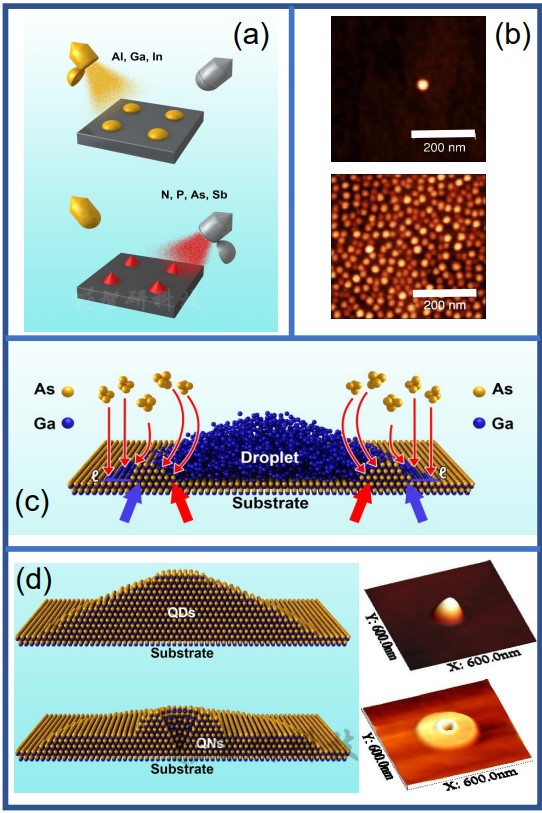
\includegraphics[width=10cm]{images/gurioli_fig1.png}
        \caption{\label{fig:gurioli1}
            Стадии капельной эпитаксии (воспроизведено из~\cite{gurioli2021}): (a) схема последовательного осаждения атомов III и V группы, (b) AFM-изображения капель с различной плотностью, (c) два механизма роста — поглощение атомов As каплей и диффузия Ga наружу, (d) формирование квантовой точки или кольца в зависимости от доминирующего механизма.}
    \end{center}
\end{figure}

Морфология образующихся структур чувствительна к ряду технологических параметров: температуре подложки, интенсивности и длительности потока компонентов, времени экспозиции, а также к типу и ориентации подложки. Это делает капельную эпитаксию не только удобным, но и гибким инструментом для целенаправленного синтеза наноструктур с заданными свойствами~\cite{sibirmovskiy2014}.

Стадии капельной эпитаксии наглядно представлены на схематическом изображении, заимствованном из статьи~\cite{gurioli2021} (рис.~\ref{fig:gurioli1}). На нём показан процесс формирования капель, возможные пути кристаллизации и типичные формы наноструктур.

Дополнительно, на рис.~\ref{fig:zhou1} представлена последовательность реальных SEM-изображений, иллюстрирующая трансформацию капли Ga во времени под действием потока As, в том числе образование двойного кольца. Эти данные наглядно подтверждают описанный выше механизм.

\begin{figure}[H]
    \begin{center}
        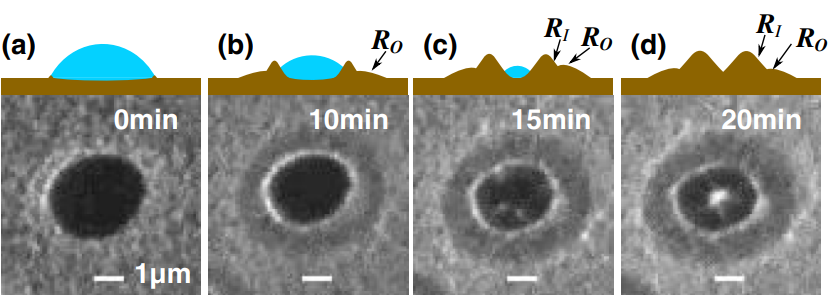
\includegraphics[width=11cm]{images/Zhou1-Firgure1.png}
        \caption{\label{fig:zhou1}
            Эволюция капли Ga и формирование квантового кольца во времени при капельной эпитаксии. Изображения получены методом MEM. Виден переход от капли к юбкообразной структуре и далее к двойному кольцу. Воспроизведено из~\cite{zhou2013}.}
    \end{center}
\end{figure}

\subsection{Квантовые кольца: геометрия, свойства, эффекты}

Квантовые кольца (КК) — это наноструктуры с тороидальной симметрией и выраженным центральным отверстием, отличающиеся от квантовых точек своей геометрией и спектром состояний. Такая топология существенно влияет на свойства локализованных в кольце электронов и дырок. В отличие от точек, где частицы локализуются в центре, в кольце они прижаты к периферии, что приводит к целому ряду квантовых эффектов.

Один из наиболее ярких эффектов — это эффект Ааронова–Бома, при котором энергетические уровни квантового кольца осциллируют в зависимости от магнитного потока, проходящего через его центр. Уравнение для энергии носителя в кольце радиуса $r$ имеет вид:

\[
E_M = \frac{\hbar^2}{2m^* r^2} \left( M + \frac{\Phi}{\Phi_0} \right)^2,
\]

где $M$ — магнитное квантовое число, $m^*$ — эффективная масса, $\Phi$ — магнитный поток, $\Phi_0 = h/e$ — квант потока.

Наличие топологического отверстия также влияет на пространственное распределение плотности состояний, запрещая плотную локализацию в центре и изменяя характер волновых функций. Это приводит к специфическим оптическим переходам: изменениям в ширине линии фотолюминесценции, поляризационной анизотропии, а также чувствительности к направлению магнитного поля~\cite{Beo2020}.

Согласно экспериментальным данным~\cite{sibirmovskiy2018}, кольца на основе GaAs/AlGaAs демонстрируют необычную температурную зависимость фотолюминесценции: при нагревании от 20 до 70 К интенсивность ФЛ растёт, а ширина линии уменьшается, что связывается с термоактивацией носителей и неоднородной формой кольца. Кроме того, благодаря высокой симметрии кольцевой формы, КК демонстрируют слабо выраженную поляризацию испускаемого света, что делает их удобными для задач квантовой фотоники.

Энергетические и оптические свойства КК зависят от их геометрических параметров — внешнего и внутреннего радиусов, толщины, глубины. Геометрия, в свою очередь, может быть определена, например, методом атомно-силовой микроскопии. На рис.~\ref{fig:elborg2} представлен AFM-изображение одиночного квантового кольца, полученного в работе~\cite{elborg2017}.

\begin{figure}[H]
    \begin{center}
        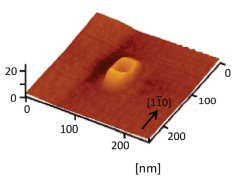
\includegraphics[width=11cm]{images/elborg_fig2.png}
        \caption{\label{fig:elborg2}
            AFM-изображения одиночного квантового кольца (вверху) и кольца с точкой в центре (внизу), полученных методом капельной эпитаксии. Воспроизведено из работы~\cite{elborg2017}.}
    \end{center}
\end{figure}

Квантовые кольца находят применение в квантовой криптографии, в качестве однофотонных источников, а также в схемах логических вентилей, использующих спиновые и орбитальные степени свободы. Их особые геометрические и магнитные свойства делают их также перспективными для реализации твердотельных квантовых битов~\cite{Liu2019}.

\subsection{Влияние условий роста на морфологию квантовых колец}

Морфология квантовых колец, формируемых методом капельной эпитаксии, определяется множеством взаимосвязанных параметров. Помимо температуры подложки и потока мышьяка, большое значение имеют: объём капли, ориентация кристаллической подложки, режим подачи компонентов, параметры десорбции и свойства мокрого слоя. Управление этими факторами позволяет синтезировать кольца с заданной формой, размерами и симметрией.

Одним из наиболее исследованных параметров является температура подложки(см. рис.~\ref{fig:morph_map}). При низких температурах ($T < 250\,^{\circ}\mathrm{C}$) ограниченная диффузия атомов Ga приводит к формированию компактных точек или толстостенных колец. При увеличении температуры ($T \approx 300\,^{\circ}\mathrm{C}$) диффузия усиливается, что способствует расширению кольца и образованию симметричной структуры. Однако при слишком высоких температурах ($T > 330\,^{\circ}\mathrm{C}$) доминирует десорбция мышьяка, что может привести к неравномерной кристаллизации и даже исчезновению кольца~\cite{sibirmovskiy2014,vasilevskiy2013}.

Интенсивность потока мышьяка (или эффективное давление As$_4$) регулирует скорость кристаллизации(см. рис.~\ref{fig:morph_map}). Высокий поток ведёт к мгновенному насыщению капли As и образованию точек. Напротив, при умеренном или ступенчатом потоке As возможно последовательное формирование двойных или концентрических колец~\cite{zhou2013,fan2023}.

\begin{figure}[H]
    \begin{center}
        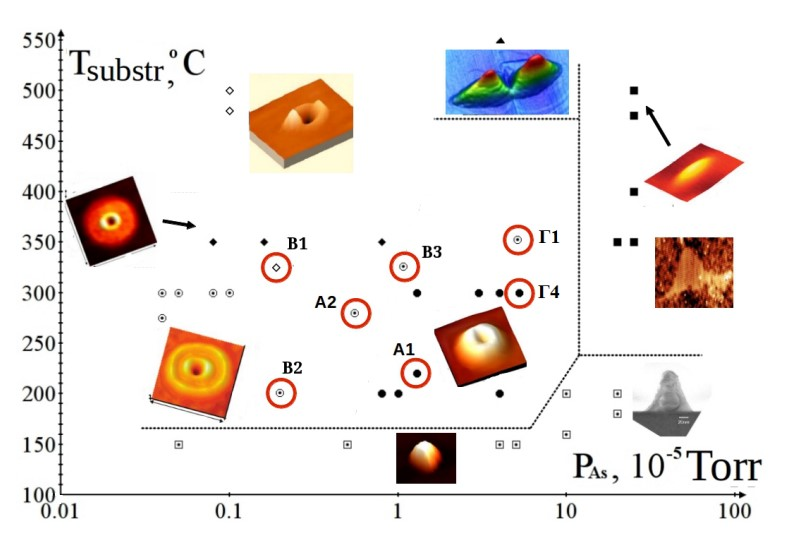
\includegraphics[width=14cm]{images/morphology_map.png}
        \caption{\label{fig:morph_map}
            Морфология квантовых колец GaAs/AlGaAs в зависимости от температуры подложки и давления мышьяка. Изображения структур заимствованы из работ~\cite{mano2005nano, koguchi2005growth, vasilevskiy2013}.}
    \end{center}
\end{figure}

Схожие результаты были получены в недавней обзорной работе Fan и Ma~\cite{fan2023}, где показано, как изменяются формы GaAs наноструктур (точки, кольца, двойные кольца, диск) при варьировании температуры и потока As. При 150 °C формируются точки, при 200 °C — кольца, а при 300 °C наблюдаются двойные кольца и кольцевые углубления (см. рис.~\ref{fig:fanma_temp}). Аналогично, при фиксированной температуре изменение потока As также приводит к трансформации форм (см. рис.~\ref{fig:fanma_pressure}).

\begin{figure}[H]
    \begin{center}
        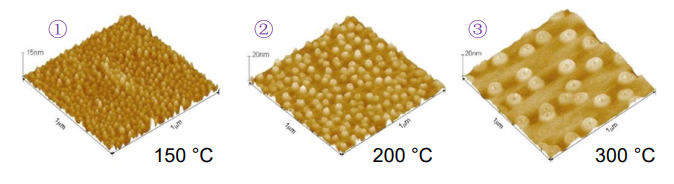
\includegraphics[width=11cm]{images/fanma_fig2e_left.png}
        \caption{\label{fig:fanma_temp}
            Изменение формы квантовых колец GaAs в зависимости от температуры. Воспроизведено из~\cite{fan2023}, рис.~2(e).}
    \end{center}
\end{figure}

\begin{figure}[H]
    \begin{center}
        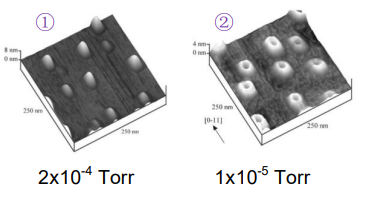
\includegraphics[width=11cm]{images/fanma_fig2e_right.png}
        \caption{\label{fig:fanma_pressure}
            Изменение формы квантовых колец GaAs в зависимости от давления мышьяка. Воспроизведено из~\cite{fan2023}, рис.~2(f).}
    \end{center}
\end{figure}

Помимо температуры подложки и потока мышьяка, на морфологию квантовых колец существенное влияние оказывают и другие параметры роста. К ним относятся:

\begin{itemize}
    \item \textbf{Объём капли Ga.} Определяет форму и ширину кольца. При малом объёме формируются узкие симметричные кольца, при увеличенном — кольца с размытыми границами или асимметрией. Существенное влияние оказывает начальный радиус и масса капли~\cite{zhou2013}.

    \item \textbf{Ориентация подложки.} На подложках GaAs(001) и GaAs(111) наблюдаются различия в симметрии кольцевых структур. Анизотропия поверхностной энергии и направленности диффузии приводит к вытягиванию кольца вдоль кристаллографических осей~\cite{elborg2017}.

    \item \textbf{Наличие смачивабщего слоя.} Если до или во время кристаллизации присутствует остаточный слой Ga или GaAs, он может «заполнять» центр кольца, делая профиль менее глубоким. В его отсутствие кольцо формируется с резкой ямой в центре~\cite{sibirmovskiy2014}.

    \item \textbf{Режим подачи мышьяка.} При непрерывной подаче формируются одиночные кольца, а при ступенчатой или импульсной — двойные и многокольцевые структуры. Режим подачи влияет на скорость кристаллизации и изменение границ капли~\cite{wang2022}.

    \item \textbf{Десорбция мышьяка.} При повышенных температурах атомы As быстро десорбируются с поверхности до завершения реакции, что может привести к неравномерной или частично разрушенной кольцевой морфологии~\cite{fan2023}.
\end{itemize}

Таким образом, морфология квантовых колец — это результат тонкого баланса между параметрами роста, диффузией, реакцией и десорбцией. Только комплексное управление этими условиями позволяет воспроизводимо получать наноструктуры с нужной формой и функциональностью.

\subsection{Современные подходы к моделированию роста квантовых колец}

Моделирование роста квантовых колец методом капельной эпитаксии остаётся активно развивающимся направлением, в котором используется широкий спектр физических и численных подходов. В данной части представлены основные классы моделей, применяемые в литературе, с анализом их возможностей и ограничений.

\subsubsection*{Модели на основе уравнений диффузии и химической реакции}
Один из наиболее распространённых подходов основан на описании эволюции поверхностных концентраций компонентов III и V групп с помощью реакционно-диффузионных уравнений. Такие модели позволяют анализировать пространственное распределение атомов и воспроизводить морфологию кольца. Классическим примером является модель, предложенная в работе Zhou et al.\cite{zhou2013}, в которой учитываются диффузия атомов Ga и As, их взаимодействие, а также влияние параметров роста. Модель хорошо воспроизводит профиль кольца, но не учитывает динамическое изменение радиуса капли. На рис.\ref{fig:zhou_profiles} показано соответствие между профилем кольца, полученным в расчёте, и экспериментальными AFM-данными.

\begin{figure}[H]
    \begin{center}
        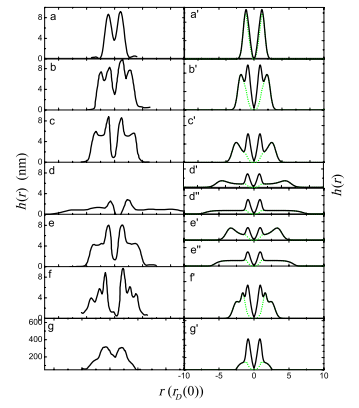
\includegraphics[width=11cm]{images/zhou_profiles.png}
        \caption{\label{fig:zhou_profiles}
            Сравнение экспериментальных (слева) и рассчитанных (справа) профилей высоты кольцевых структур GaAs. Воспроизведено из~\cite{zhou2013}, рис.~4.}
    \end{center}
\end{figure}

\subsubsection*{Кинетические модели нуклеации и эволюции капель}
Другим направлением являются модели, описывающие образование и эволюцию капель на подложке. Они фокусируются на стадиях нуклеации, росте и слиянии капель, а также на влиянии температуры и плотности потока. Модель Dubrovskii et al.\cite{dubrovskii2021} представляет собой систему обыкновенных дифференциальных уравнений для плотностей мономеров, капель и критического размера. Она позволяет количественно описать начальную стадию формирования кольца, однако не рассматривает морфологию полученной структуры. На рис.\ref{fig:dubrovskii_model} показана временная эволюция параметров нуклеации согласно расчётам данной модели.

\begin{figure}[H]
    \begin{center}
        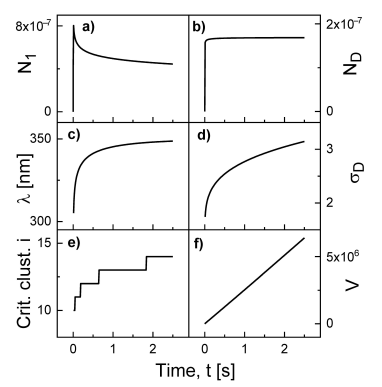
\includegraphics[width=11cm]{images/dubrovskii_fig2.png}
        \caption{\label{fig:dubrovskii_model}
            Временная эволюция параметров нуклеации и роста капли: (a--f) — плотность мономеров, плотность капель, длина диффузии, число захвата, критический размер, объём капли. Воспроизведено из~\cite{dubrovskii2021}, рис.~2.}
    \end{center}
\end{figure}

\subsubsection*{Модели на основе метода Монте-Карло}
Для описания сложной кинетики роста на атомарном уровне применяются модели на основе кинетического Монте-Карло. Они позволяют учитывать локальные процессы осаждения, поверхностной диффузии и кристаллизации. Примером служит модель Shwartz et al.\cite{shwartz2018}, в которой смоделировано образование кольца с учётом направления поступления атомов As, перераспределения Ga и влияния геометрии капли. Такие модели хорошо воспроизводят эволюцию формы, но являются вычислительно затратными и трудны для параметрического анализа. На рис.\ref{fig:shwartz4} приведены последовательные конфигурации кольца на различных стадиях роста.

\begin{figure}[H]
    \begin{center}
        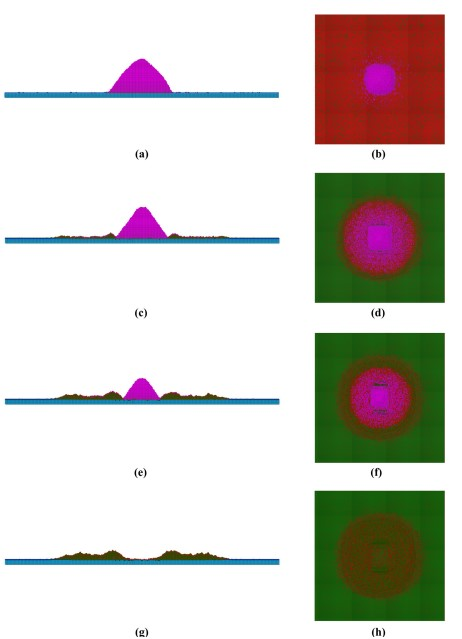
\includegraphics[width=9cm]{images/shwartz_fig4.png}
        \caption{\label{fig:shwartz4}
            Эволюция морфологии кольца в модели Монте-Карло. Слева — поперечные сечения, справа — вид сверху. Капля Ga обозначена фиолетовым, GaAs — коричневым. Воспроизведено из~\cite{shwartz2018}, рис.~4.}
    \end{center}
\end{figure}

\subsubsection*{Сравнительный анализ подходов}
Все рассмотренные модели акцентируют внимание на различных аспектах роста кольца. Диффузионно-реакционные модели эффективны при анализе морфологии, но чувствительны к выбору граничных условий. Кинетические уравнения нуклеации хорошо описывают начальную стадию, но не дают информации о форме. Модели Монте-Карло подходят для анализа атомарных механизмов, но требуют большого объёма вычислений.

Для целей данной работы необходимо было объединить преимущества разных подходов: описать как пространственную структуру концентраций, так и изменение геометрии капли во времени. Поэтому была выбрана гибридная модель, сочетающая диффузию, химию и динамику радиуса — подробнее она представлена в следующем разделе.

\subsection{Обоснование выбора подхода к моделированию}

Анализ существующих моделей показывает, что каждая из них решает строго ограниченную задачу: описывает либо морфологию кольца при фиксированных условиях, либо начальную стадию нуклеации капли, либо пространственно-атомарную кинетику. Однако ни одна из них не объединяет в себе:

\begin{itemize}
  \item динамическое изменение радиуса капли;
  \item пространственно-временное распределение концентраций Ga и As;
  \item рост высоты кольца как результат поверхностной реакции;
  \item физически обоснованное распределение потока галлия из капли.
\end{itemize}

В связи с этим в рамках данной работы была разработана модель, сочетающая принципы реакционно-диффузионного описания, приближённое уравнение эволюции радиуса капли, численное описание роста кольца и гауссов профиль потока. Такая постановка позволяет анализировать влияние параметров роста на морфологию кольца и служит основой для построения численной схемы.

Подробное описание модели и всех входящих уравнений приводится в следующей главе.


% ============================================
% ГЛАВА 2
% ============================================
\pagebreak

\section{Физико-математическая модель}

\subsection{Основные уравнения диффузии и реакций}

Процесс формирования кольцевой структуры при капельной эпитаксии можно описывать с помощью реакционно-диффузионной модели в предположении осевой симметрии. Подобные модели применяются в ряде современных исследований~\cite{reyes2013, bietti2020}, позволяя анализировать пространственно-временное распределение компонентов и их взаимодействие на поверхности.

Пусть $c_{\text{Ga}}(r,t)$ и $c_{\text{As}}(r,t)$ — поверхностные концентрации атомов галлия и мышьяка соответственно, зависящие от радиальной координаты $r$ и времени $t$.

Для обоих компонентов учитываются диффузия, поступление вещества (для As — постоянный поток, для Ga — гауссов профиль из капли), а также реакция между ними, приводящая к образованию твёрдой фазы GaAs. Для мышьяка дополнительно учитывается десорбция с поверхности.

Такой подход описан, в частности, в работе~\cite{reyes2013_1}, где предложена численная модель, объединяющая кинетические и диффузионные аспекты. В другом исследовании~\cite{bietti2020} показано, как изменение потока мышьяка и температуры влияет на соотношение между объёмами GaAs, кристаллизующегося внутри капли и по её границе.

Уравнения системы имеют следующий вид:

\begin{equation}
\frac{\partial C_{Ga}}{\partial t}=D_{Ga}\frac{1}{r}\frac{\partial}{\partial r}\left(r\frac{\partial C_{Ga}}{\partial r}\right)+F_{Ga}\left(r,t\right)-k_{r}C_{Ga}C_{As}
\label{eq:ga_diff}
\end{equation}

\begin{equation}
\frac{\partial C_{As}}{\partial t}=D_{As}\frac{1}{r}\frac{\partial}{\partial r}\left(r\frac{\partial C_{As}}{\partial r}\right)+F_{As}-k_{r}C_{Ga}C_{As}-\frac{C_{As}}{\tau_{As}},
\label{eq:as_diff}
\end{equation}

где:
\begin{itemize}
  \item $D_{\text{Ga}}, D_{\text{As}}$ — коэффициенты поверхностной диффузии;
  \item $k_{r}$ — коэффициент реакции между атомами Ga и As;
  \item $F_{\text{As}}$ — постоянный поток мышьяка;
  \item $F_{\text{Ga}}(r,t)$ — пространственно и временно зависимый поток галлия;
  \item $\tau_{\text{As}}$ — характерное время десорбции мышьяка.
\end{itemize}

\begin{equation}
D_{Ga}=a_{0}^{2}\nu\exp\left(-\frac{E_{Ga}}{kT}\right)
\end{equation}

\begin{equation}
D_{As}=a_{0}^{2}\nu\exp\left(-\frac{E_{As}}{kT}\right)
\end{equation}

Время десорбции мышьяка:

\begin{equation}
\tau_{As}=\frac{1}{\nu}\exp\left(\frac{E_{a}}{kT}\right)
\end{equation}

\begin{equation}
\nu=\frac{kT}{\pi\hbar}
\end{equation}

Модель использует приближение сплошной среды, что оправдано для масштабов порядка десятков нанометров. Она позволяет изучать влияние параметров роста на морфологию кольца в рамках эффективной численной реализации.

Модель задаётся на интервале $r \in [0, R_\infty]$ с осевой симметрией. Поверхностные концентрации атомов $C_{\text{Ga}}(r,t)$ и $C_{\text{As}}(r,t)$ описываются уравнениями~\eqref{eq:ga_diff}–\eqref{eq:as_diff}, и для их корректного численного решения необходимо задать начальные и граничные условия.

\subsubsection*{Начальные условия}

На начальный момент времени ($t = 0$): 

\begin{equation}
C_{Ga}\left(r,0\right)=0, \qquad
C_{As}\left(r,0\right)=0.
\end{equation}

\subsubsection*{Граничные условия}

На правой границе области ($r = R_\infty$) задаются:

\begin{equation}
C_{Ga}\left(R_{\infty},t\right)=0, \qquad
C_{As}\left(R_{\infty},t\right)=F_{As}\tau_{As}.
\end{equation}

\subsection{Распределение потока галлия из капли}

Одним из ключевых элементов модели капельной эпитаксии является описание пространственного распределения потока галлия, поступающего из жидкой капли на подложку. Корректное задание этой функции необходимо для воспроизведения морфологии кольца и скорости роста наноструктуры. Ниже приведено подробное аналитическое построение соответствующего выражения, опирающееся на решение уравнения диффузии с заданными граничными условиями.

\begin{figure}[H]
    \begin{center}
        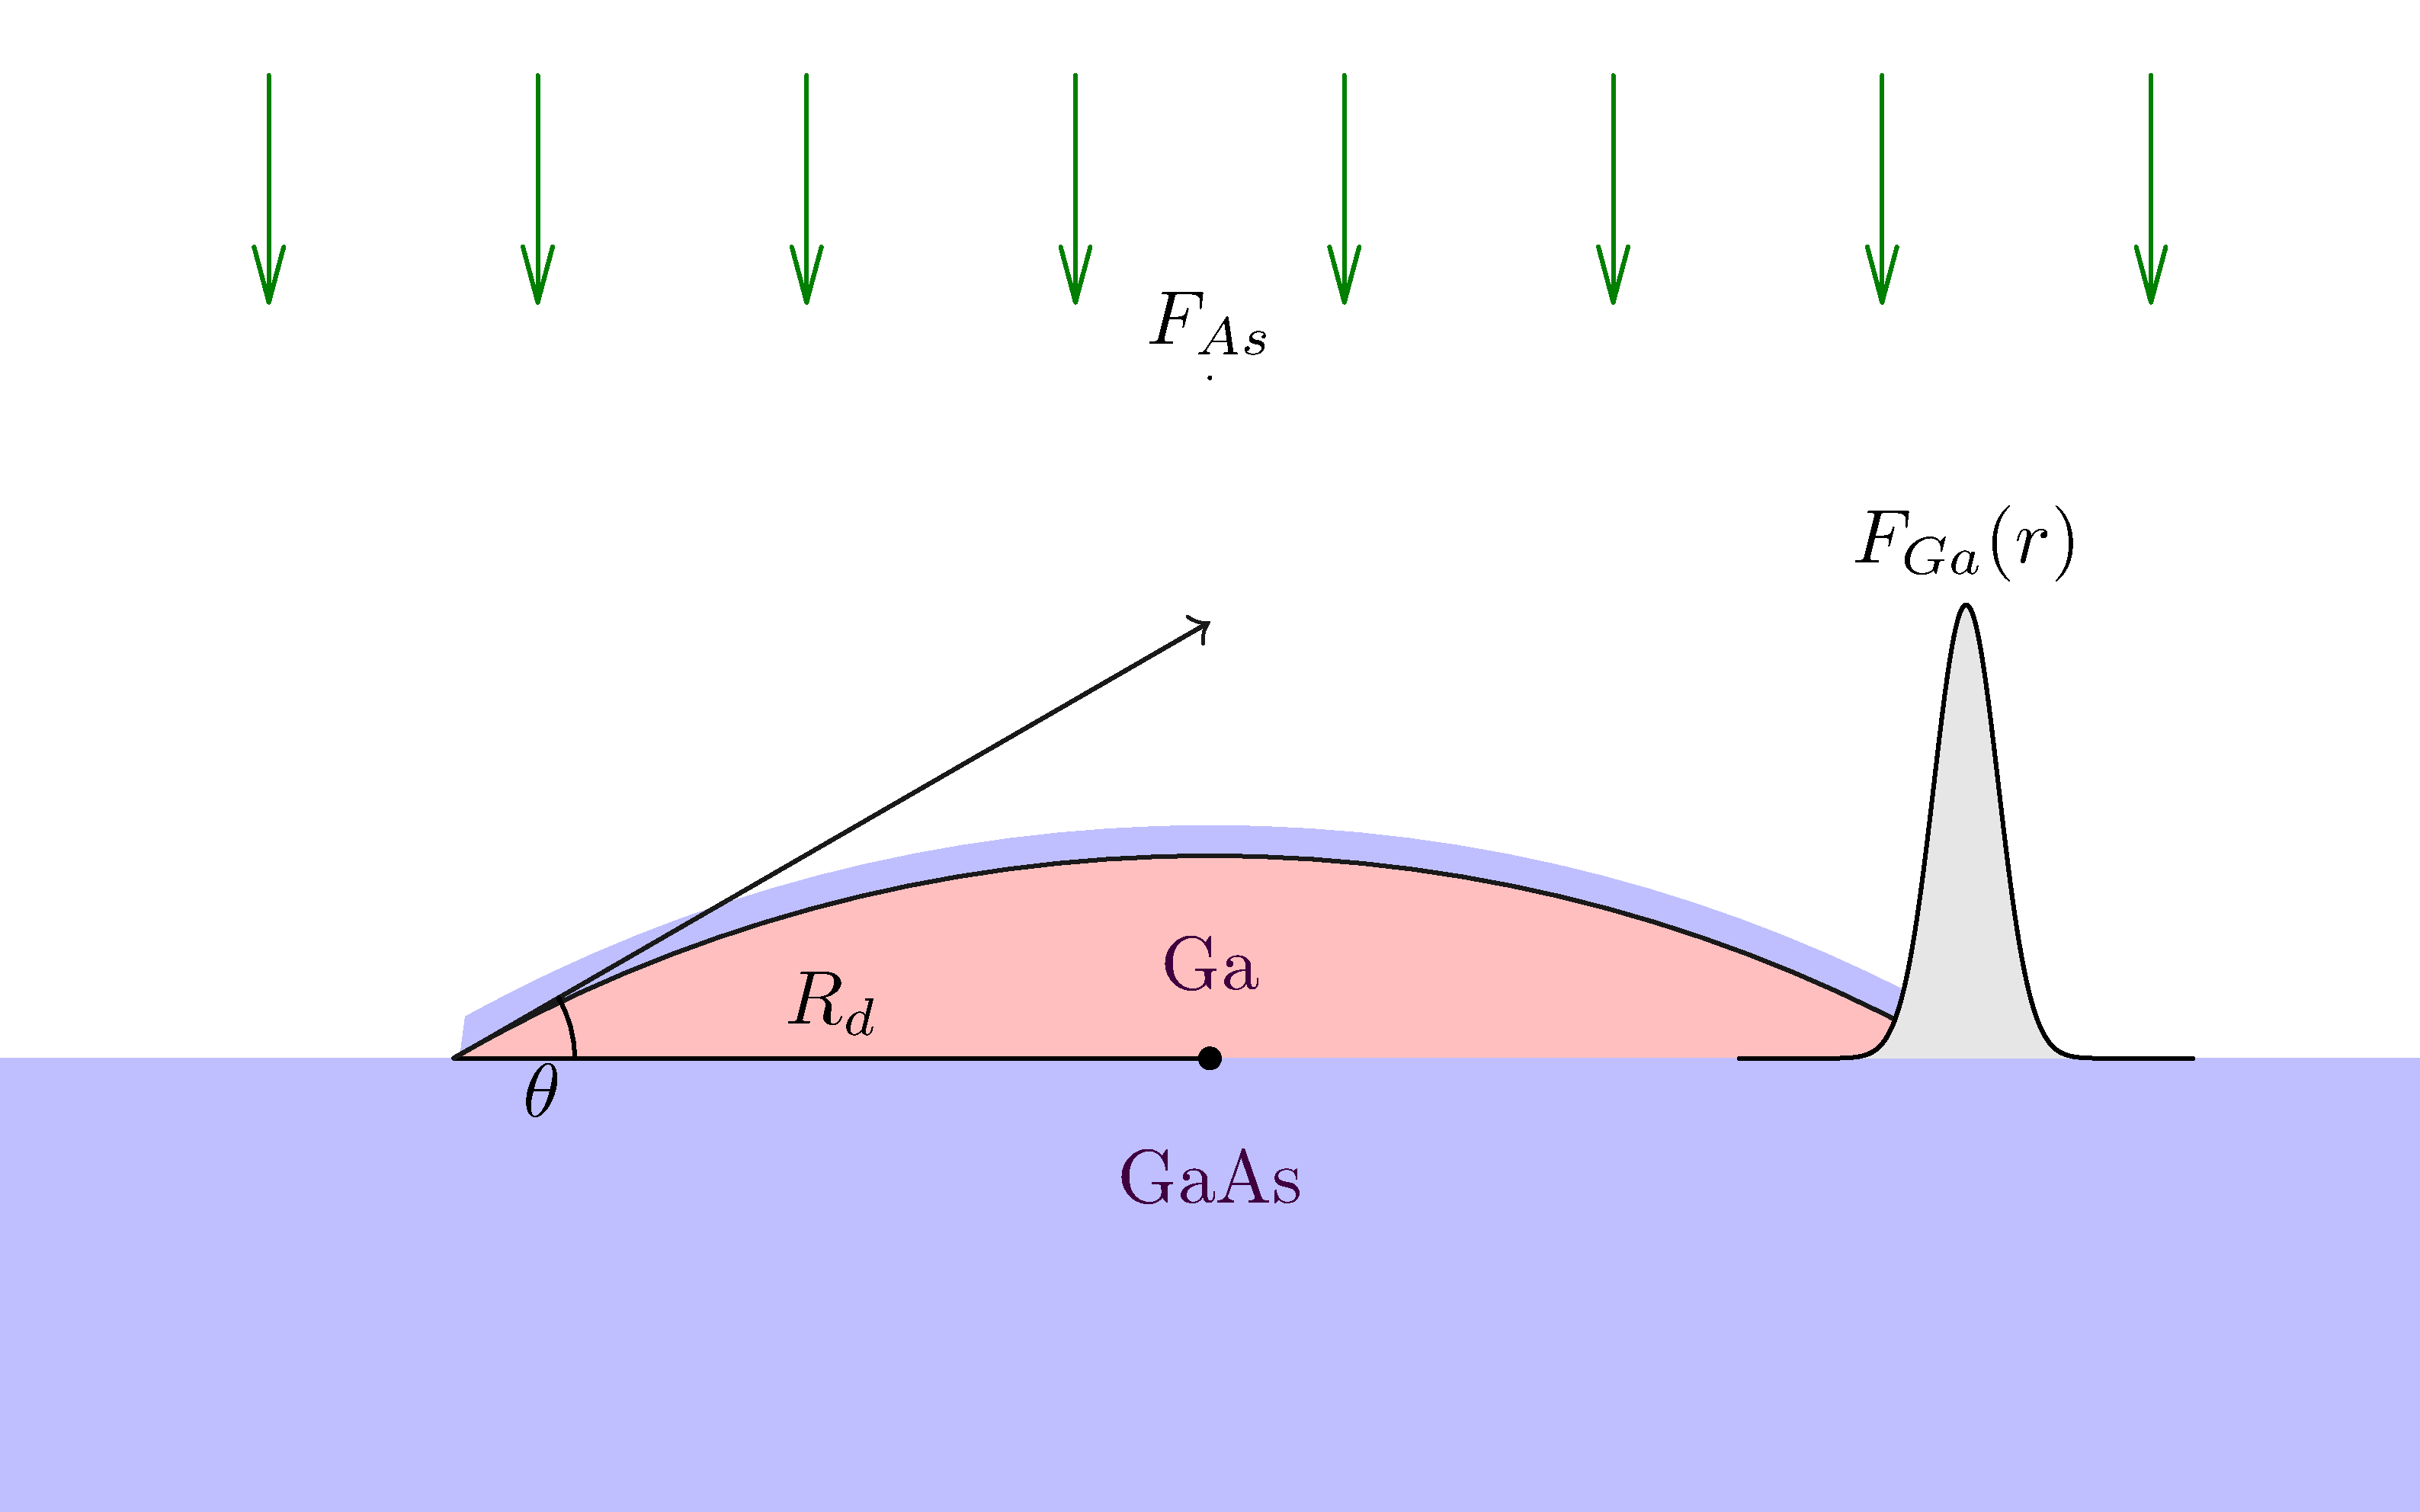
\includegraphics[width=11cm]{images/first.png}
        \caption{\label{fig:first}
        Визуализация потоков Ga}
    \end{center}
\end{figure}

Общее выражение для потока (рис.~\ref{fig:first}):

\begin{equation}
    F_{Ga}\left(r,t\right)=\frac{C_{0}}{\tau_{Ga}\left(t\right)}\exp\left(-\frac{\left(r-R_{d}\left(t\right)\right)^{2}}{w^{2}}\right)
\end{equation}

Мы решаем упрощённую задачу о капле Ga, испускающей атомы в присутствии потока As, и предполагаем сильное взаимодействие, при котором каждый поступающий атом As удаляет один атом Ga с поверхности, связывая его и образуя GaAs. Тогда уравнение диффузии для Ga будет выглядеть так:

\begin{equation}
    \frac{\partial C_{Ga}}{\partial t}=D_{Ga}\frac{1}{r}\frac{\partial}{\partial r}\left(r\frac{\partial C_{Ga}}{\partial r}\right)-F_{As}
\end{equation}

\[
C_{Ga}\left(R_{d},t\right)=C_{0}
\]

\[
C_{Ga}\left(R_{\infty},t\right)=0
\]

Давайте решим задачу, предположив, что состояние стационарно:

\[
\frac{\partial C_{Ga}}{\partial t}=0
\]

\[
\frac{1}{r}\frac{\partial}{\partial r}\left(r\frac{\partial C_{Ga}}{\partial r}\right)=\frac{F_{As}}{D_{Ga}}
\]

Общее решение таково:

\[
C_{Ga}=\frac{F_{As}}{4D_{Ga}}r^{2}+A\ln\frac{r}{a}
\]

где A, a — неизвестные константы.

Чтобы вычислить их, мы используем граничные условия.

Первое граничное условие:

\[
\frac{F_{As}}{4D_{Ga}}R_{d}^{2}+A\ln\frac{R_{d}}{a}=C_{0}\qquad\Rightarrow\qquad A=\frac{C_{0}-\frac{F_{As}}{4D_{Ga}}R_{d}^{2}}{\ln\frac{R_{d}}{a}}
\]

Обозначим:

\begin{equation}
    \frac{F_{As}R_{d}^{2}}{4D_{Ga}}=C_{d}
\end{equation}

\[
C_{Ga}=C_{d}\frac{r^{2}}{R_{d}^{2}}+\left(C_{0}-C_{d}\right)\frac{\ln\frac{r}{a}}{\ln\frac{R_{d}}{a}}=C_{d}\left(\frac{r^{2}}{R_{d}^{2}}+\left(\frac{C_{0}}{C_{d}}-1\right)\frac{\ln\frac{r}{a}}{\ln\frac{R_{d}}{a}}\right)
\]
  
Снова проверяем граничные условия:

\[
C_{Ga}\left(R_{d}\right)=C_{d}\left(1+\frac{C_{0}}{C_{d}}-1\right)=C_{0}
\]

Второе граничное условие:

\begin{multline*}
    C_{d}\left(
    \frac{R_{\infty}^{2}}{R_{d}^{2}} +
    \left(\frac{C_{0}}{C_{d}} - 1\right)
    \cdot
    \frac{\ln\left( \frac{R_{\infty}}{a} \right)}{\ln\left( \frac{R_{d}}{a} \right)}
    \right)
    = 0
    \qquad\Rightarrow\qquad \\
    \left(\ln R_{d} - \ln a\right)
    \cdot \frac{R_{\infty}^{2}}{R_{d}^{2}} =
    -\left( \frac{C_{0}}{C_{d}} - 1 \right)
    \cdot \left(\ln R_{\infty} - \ln a\right)
\end{multline*}
    

\[
\left(\frac{C_{0}}{C_{d}}-1+\frac{R_{\infty}^{2}}{R_{d}^{2}}\right)\ln a=\frac{R_{\infty}^{2}}{R_{d}^{2}}\ln R_{d}+\left(\frac{C_{0}}{C_{d}}-1\right)\ln R_{\infty}
\]

\[
\ln a=\frac{\frac{R_{\infty}^{2}}{R_{d}^{2}}\ln R_{d}+\left(\frac{C_{0}}{C_{d}}-1\right)\ln R_{\infty}}{\frac{C_{0}}{C_{d}}-1+\frac{R_{\infty}^{2}}{R_{d}^{2}}}
\]

Итак, мы получаем:

\begin{multline*}
    \ln R_{d} - \ln a =
    \frac{
    \left( \frac{C_0}{C_d} - 1 \right) \ln R_d
    + \frac{R_{\infty}^{2}}{R_d^2} \ln R_d
    - \frac{R_{\infty}^{2}}{R_d^2} \ln R_d
    - \left( \frac{C_0}{C_d} - 1 \right) \ln R_{\infty}
    }{
    \left( \frac{C_0}{C_d} - 1 \right)
    + \frac{R_{\infty}^{2}}{R_d^2}
    } = \\
    = \frac{
    \left( \frac{C_0}{C_d} - 1 \right)
    }{
    \left( \frac{C_0}{C_d} - 1 \right)
    + \frac{R_{\infty}^{2}}{R_d^2}
    }
    \cdot \ln \left( \frac{R_d}{R_{\infty}} \right)
\end{multline*}
    
\begin{multline*}
    \ln R_{\infty} - \ln a =
    \frac{
    \left( \frac{C_0}{C_d} - 1 \right) \ln R_{\infty}
    + \frac{R_{\infty}^2}{R_d^2} \ln R_{\infty}
    - \frac{R_{\infty}^2}{R_d^2} \ln R_d
    - \left( \frac{C_0}{C_d} - 1 \right) \ln R_{\infty}
    }{
    \left( \frac{C_0}{C_d} - 1 \right) + \frac{R_{\infty}^2}{R_d^2}
    } = \\
    = -\frac{ \dfrac{R_{\infty}^2}{R_d^2} }{ 
    \left( \dfrac{C_0}{C_d} - 1 \right) + \dfrac{R_{\infty}^2}{R_d^2} 
    }
    \cdot \ln \left( \frac{R_d}{R_{\infty}} \right)
\end{multline*}
    
   
Так:

\[
\ln\frac{r}{a}=\ln\frac{r}{R_{\infty}}+\ln\frac{R_{\infty}}{a}=\ln\frac{r}{R_{\infty}}-\frac{\frac{R_{\infty}^{2}}{R_{d}^{2}}}{\frac{C_{0}}{C_{d}}-1+\frac{R_{\infty}^{2}}{R_{d}^{2}}}\ln\frac{R_{d}}{R_{\infty}}
\]

И так мы имеем:

\[
C_{Ga}=C_{d}\left(\frac{r^{2}}{R_{d}^{2}}+\frac{\left(\frac{C_{0}}{C_{d}}-1+\frac{R_{\infty}^{2}}{R_{d}^{2}}\right)\ln\frac{r}{R_{\infty}}-\frac{R_{\infty}^{2}}{R_{d}^{2}}\ln\frac{R_{d}}{R_{\infty}}}{\ln\frac{R_{d}}{R_{\infty}}}\right)
\]

Упрощаем:

\begin{equation}
    C_{Ga}=C_{d}\left(\frac{r^{2}-R_{\infty}^{2}}{R_{d}^{2}}+\left(\frac{C_{0}}{C_{d}}-1+\frac{R_{\infty}^{2}}{R_{d}^{2}}\right)\frac{\ln\frac{r}{R_{\infty}}}{\ln\frac{R_{d}}{R_{\infty}}}\right)
\end{equation}

\[
C_{d}=\frac{F_{As}R_{d}^{2}}{4D_{Ga}}
\]

Проверка второго граничного условия не представляет сложности. 

Теперь снова проверим первое граничное условие:

\begin{multline*}
    C_{Ga}(R_d) = C_d \left(
    \frac{R_d^2 - R_{\infty}^2}{R_d^2}
    + \left(
    \frac{C_0}{C_d} - 1 + \frac{R_{\infty}^2}{R_d^2}
    \right)
    \cdot
    \frac{ \ln \left( \frac{R_d}{R_{\infty}} \right) }{ \ln \left( \frac{R_d}{R_{\infty}} \right) }
    \right) = \\
    = C_d \left(
    1 - \frac{R_{\infty}^2}{R_d^2}
    + \left( \frac{C_0}{C_d} - 1 + \frac{R_{\infty}^2}{R_d^2} \right)
    \right) = C_0
\end{multline*}
    

Теперь нам нужно найти поток на границе капли:

\begin{equation}
    J_{Ga}=-D_{Ga}\frac{\partial C_{Ga}}{\partial r}\left(r=R_{d}\right)
\end{equation}

\begin{multline}
    \left. \frac{\partial C_{\text{Ga}}}{\partial r} \right|_{r = R_d}
    = C_d \left(
    \frac{2r}{R_d^2}
    + \frac{ \frac{C_0}{C_d} - 1 + \frac{R_\infty^2}{R_d^2} }{ \ln \left( \frac{R_d}{R_\infty} \right) } \cdot \frac{1}{r}
    \right) \Bigg|_{r = R_d} = \\
    = -\frac{2C_d}{R_d} \left(
    \frac{
    \frac{C_0}{C_d} - 1 + \frac{R_\infty^2}{R_d^2}
    }{
    2 \ln \left( \frac{R_\infty}{R_d} \right)
    }
    - 1
    \right) < 0
\end{multline} 

Последнее условие вытекает из общего неравенства $x^{2}+\epsilon>\ln x^{2}$,  $x\geq1$ и:

\[
\frac{C_{0}}{C_{d}}-1+\frac{R_{\infty}^{2}}{R_{d}^{2}}>2\ln\frac{R_{\infty}}{R_{d}}=\ln\frac{R_{\infty}^{2}}{R_{d}^{2}},\qquad C_{0}>C_{d}
\]

Отрицательный поток подтверждает, что концентрация Ga уменьшается по мере удаления от капли, как и должно быть.

\begin{equation}
    J_{Ga}=\frac{2C_{d}D_{Ga}}{R_{d}}\left(\frac{\frac{C_{0}}{C_{d}}-1+\frac{R_{\infty}^{2}}{R_{d}^{2}}}{2\ln\frac{R_{\infty}}{R_{d}}}-1\right)=\frac{F_{As}R_{d}}{2}\left(\frac{\frac{C_{0}}{C_{d}}-1+\frac{R_{\infty}^{2}}{R_{d}^{2}}}{2\ln\frac{R_{\infty}}{R_{d}}}-1\right)
\end{equation}

Таким образом, мы получаем:

\begin{equation}
    \frac{dN_{Ga}}{dt}=-2\pi R_{d}J_{Ga}=-\pi F_{As}R_{d}^{2}\left(\frac{\frac{C_{0}}{C_{d}}-1+\frac{R_{\infty}^{2}}{R_{d}^{2}}}{2\ln\frac{R_{\infty}}{R_{d}}}-1\right)
\end{equation}

\begin{equation}
    \frac{dN_{Ga}}{dt}=-\pi\frac{C_{0}w^{2}}{\tau_{Ga}}\left[\exp\left(-\frac{R_{d}^{2}}{w^{2}}\right)+\sqrt{\pi}\frac{R_{d}}{w}\left\{ 1+\text{erf}\left(\frac{R_{d}}{w}\right)\right\} \right]
\end{equation}

Сравнивая эти два выражения, мы получаем:

\[
F_{As}R_{d}^{2}\left(\frac{\frac{C_{0}}{C_{d}}-1+\frac{R_{\infty}^{2}}{R_{d}^{2}}}{2\ln\frac{R_{\infty}}{R_{d}}}-1\right)=\frac{C_{0}w^{2}}{\tau_{Ga}}\left[\exp\left(-\frac{R_{d}^{2}}{w^{2}}\right)+\sqrt{\pi}\frac{R_{d}}{w}\left\{ 1+\text{erf}\left(\frac{R_{d}}{w}\right)\right\} \right]
\]

\[
\tau_{Ga}=\frac{C_{0}w^{2}}{F_{As}R_{d}^{2}}\frac{\exp\left(-\frac{R_{d}^{2}}{w^{2}}\right)+\sqrt{\pi}\frac{R_{d}}{w}\left\{ 1+\text{erf}\left(\frac{R_{d}}{w}\right)\right\} }{\frac{\frac{C_{0}}{C_{d}}-1+\frac{R_{\infty}^{2}}{R_{d}^{2}}}{2\ln\frac{R_{\infty}}{R_{d}}}-1}
\]

\begin{equation}
    F_{Ga}\left(r,t\right)=F_{As}\frac{R_{d}^{2}}{w^{2}}\frac{\left(\frac{\frac{C_{0}}{C_{d}}-1+\frac{R_{\infty}^{2}}{R_{d}^{2}}}{2\ln\frac{R_{\infty}}{R_{d}}}-1\right)\exp\left(-\frac{\left(r-R_{d}\left(t\right)\right)^{2}}{w^{2}}\right)}{\exp\left(-\frac{R_{d}^{2}}{w^{2}}\right)+\sqrt{\pi}\frac{R_{d}}{w}\left\{ 1+\text{erf}\left(\frac{R_{d}}{w}\right)\right\} }
\end{equation}

\[
C_{d}=\frac{F_{As}R_{d}^{2}}{4D_{Ga}}
\]

Или, используя приближение, описанное выше:

\[
F_{Ga}\left(r,t\right)=F_{As}\frac{R_{d}^{2}}{w^{2}}\frac{\left(\frac{\frac{C_{0}}{C_{d}}-1+\frac{R_{\infty}^{2}}{R_{d}^{2}}}{2\ln\frac{R_{\infty}}{R_{d}}}-1\right)\exp\left(-\frac{\left(r-R_{d}\left(t\right)\right)^{2}}{w^{2}}\right)}{3.545\frac{R_{d}}{w}+\frac{0.187w}{R_{\infty}-3.156w}}
\]

Давайте выделим $R_{d}$ отдельно, поскольку это функция, зависящая от времени:

\[
\frac{C_{0}}{C_{d}}=\frac{4D_{Ga}C_{0}}{F_{As}R_{d}^{2}}
\]

\begin{equation}
    F_{Ga}\left(r,t\right)=\frac{F_{As}}{w^{2}}\frac{\left(\frac{2D_{Ga}C_{0}}{F_{As}}+\frac{R_{\infty}^{2}-R_{d}^{2}}{2}-R_{d}^{2}\ln\frac{R_{\infty}}{R_{d}}\right)\exp\left(-\frac{\left(r-R_{d}\left(t\right)\right)^{2}}{w^{2}}\right)}{\left(3.545\frac{R_{d}}{w}+\frac{0.187w}{R_{\infty}-3.156w}\right)\ln\frac{R_{\infty}}{R_{d}}}
\end{equation}

\subsection{Геометрия капли и коэффициент $B(\theta)$}

Для корректного описания изменения объёма жидкой капли галлия при капельной эпитаксии используется приближение сферического сегмента с фиксированным углом смачивания $\theta$. Такая капля рассматривается как часть сферы радиуса $R$, с высотой $h$ и радиусом основания $R_d$ (см. рис.~\ref{fig:drop_geom}).

\begin{figure}[H]
    \begin{center}
    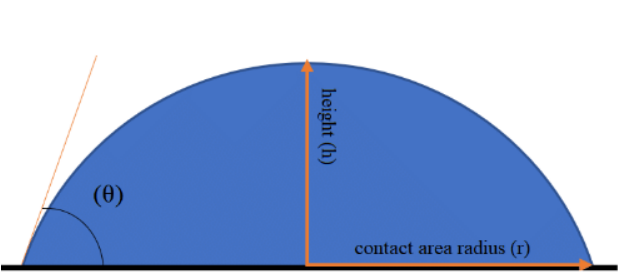
\includegraphics[width=11cm]{images/contact_angle_schematic.png}
    \caption{\label{fig:drop_geom}
    Геометрия сферической капли: $r(R_d)$ — радиус контактной области, $h$ — высота, $\theta$ — угол смачивания. Воспроизведено из работы~\cite{aboubakri2021}.}
    \end{center}
\end{figure}

Классическая формула объёма сферического сегмента имеет вид:
\begin{equation}
V = \frac{1}{3} \pi h^2 (3R - h),
\end{equation}

\[
sin\theta = \frac{R_d}{R}
\qquad
ctg\theta = \frac{R-h}{R_d}
\]

откуда $h = R(1 - \cos\theta)$.

Подставим:
\[
V = \frac{1}{3} \pi R^3 (1 - \cos\theta)^2 (2 + \cos\theta).
\]

Поскольку $R = R_d / \sin\theta$, то $R^3 = R_d^3 / \sin^3\theta$. Подставим это в выражение для $V$:
\[
V = \frac{1}{3} \pi \cdot \frac{R_d^3}{\sin^3 \theta} \cdot (1 - \cos\theta)^2 (2 + \cos\theta).
\]

Теперь введём коэффициент $B(\theta)$:
\begin{equation}
V = \frac{B(\theta)\pi R_d^3}{3}.
\end{equation}
Сравнивая, получаем:
\[
B(\theta) = \frac{\left(1-\cos\theta\right)^{2}\left(2+\cos\theta\right)}{\sin^{3}\theta}.
\]

Это выражение можно упростить до более компактной формы с использованием тригонометрических тождеств:
\[
\frac{\left(1-\cos\theta\right)^{2}\left(2+\cos\theta\right)}{\sin^{3}\theta}=\frac{\left(1-2\cos\theta+\cos^{2}\theta\right)\left(2+\cos\theta\right)}{\sin^{3}\theta}=
\]

\[
=\frac{2-4\cos\theta+2\cos^{2}\theta+\cos\theta-2\cos^{2}\theta+\cos^{3}\theta}{\sin^{3}\theta}=
\]

\[
=\frac{2-3\cos\theta+\frac{3}{4}\cos\theta+\frac{1}{4}\cos3\theta}{\frac{3}{4}\sin\theta-\frac{1}{4}\sin3\theta}=\frac{8-9\cos\theta+\cos3\theta}{3\sin\theta-\sin3\theta}
\]

\begin{equation}
B(\theta) = \frac{8-9\cos\theta+\cos3\theta}{3\sin\theta-\sin3\theta}
.
\label{eq:Btheta_final}
\end{equation}

Именно это выражение реализовано в численном коде и используется во всех вычислениях, связанных с объёмом капли.

\subsection{Рост кольца}

Рост квантового кольца происходит в результате поверхностной реакции между атомами галлия и мышьяка, приводящей к образованию кристаллической фазы GaAs. Локальное увеличение высоты кольца напрямую связано с числом образованных ячеек кристалла в данной точке.

Концентрация обоих типов атомов, связанных друг с другом и участвующих в росте кристалла, изменяется в соответствии с:

\[
\frac{dC_{\text{bound}}}{dt} = k_r \, C_{\text{Ga}}(r,t) \cdot C_{\text{As}}(r,t)
\]
где:
\begin{itemize}
  \item $C_{\text{bound}}$ — концентрация результата реакции (GaAs);
  \item $k_r$ — константа скорости реакции;
  \item $C_{\text{Ga}}, C_{\text{As}}$ — локальные концентрации атомов;
\end{itemize}

Количество вертикальных кристаллических ячеек GaAs на каждом расстоянии увеличивается в зависимости от:

\[
C_{\text{bound}} = N_{\text{cells}} \cdot C_0 \quad \Rightarrow \quad
\frac{dN_{\text{cells}}}{dt} = \frac{k_r}{C_0} \, C_{\text{Ga}} \cdot C_{\text{As}}.
\]
где:
\begin{itemize}
  \item $C_0 = \frac{1}{a_0^2}$ , $a_0$ - постоянная решётки GaAs;
  \item $N_{\text{cells}}$ — количество слоёв ячеек GaAs, выросших в данной точке (вдоль вертикали);
\end{itemize}

Высота слоя связана с этим количеством ячеек:

\[
    h=h_{0}N_{\text{cells}}
\]

\[
\frac{dh\left(r,t\right)}{dt}=\frac{h_{0}k_{r}}{C_{0}}C_{Ga}C_{As}
\]
где $h_0=a_0$ — высота одного элементарного слоя (порядка постоянной решётки);

Интегрируя это уравнение по времени, можно получить полный профиль кольца. Поскольку значения $C_{\text{Ga}}$ и $C_{\text{As}}$ варьируются по координате $r$ и времени $t$, итоговая форма кольца чувствительна к условиям роста, включая поток, температуру и геометрию капли.

\subsection{Уравнение изменения радиуса капли \texorpdfstring{$R_d(t)$}{Rd(t)}}

Изменение радиуса жидкой капли галлия во времени связано с постепенной кристаллизацией GaAs в результате взаимодействия атомов Ga и As на поверхности.
\begin{equation}
\frac{\partial C_{\text{bound}}}{\partial t}=k_{r}C_{Ga}C_{As}
\end{equation}

Это должен быть единственный способ, которым атомы Ga могут исчезнуть (за исключением тех, которые выходят за пределы границы, но мы пока отбросим их). 

Скорость изменения объёма капли пропорциональна количеству атомов, покидающих её в результате химической реакции. Если \( C_{\text{Ga}}(r,t) \) и \( C_{\text{As}}(r,t) \) — локальные поверхностные концентрации атомов галлия и мышьяка, то число атомов, вовлечённых в рост GaAs на малом интервале времени \( dt \), определяется как:

\begin{equation}
\frac{dN_{Ga}}{dt}=-2\pi k_{r}C_{0}^{2}\int_{0}^{R_{\infty}}rC_{Ga}C_{As}dr
\end{equation}

Рассмотрим сферическую каплю объёмом
\begin{equation}
V = \frac{B(\theta)\pi R_d^3}{3},
\end{equation}

Дифференцируя объём по времени, получаем:
\begin{equation}
\frac{dV}{dt} = {\pi R_d^2B(\theta)} \cdot \frac{dR_d}{dt}.
\label{eq:dVdt_from_R}
\end{equation}

С другой стороны, объём капли можно выразить через количество атомов галлия:
\begin{equation}
V = \Omega_{\text{Ga}} \cdot N_{\text{Ga}} \quad \Rightarrow \quad \frac{dV}{dt} = \Omega_{\text{Ga}} \cdot \frac{dN_{\text{Ga}}}{dt},
\label{eq:dVdt_from_N}
\end{equation}
где $\Omega_{\text{Ga}} = a_0^3$ — объём одного атома галлия.

Подставляя \eqref{eq:dVdt_from_N} в \eqref{eq:dVdt_from_R}, получаем:
\begin{equation}
\frac{dR_d}{dt} = \frac{\Omega_{\text{Ga}} }{\pi R_d^2 B(\theta)} \cdot \frac{dN_{\text{Ga}}}{dt}.
\end{equation}

Мы получаем:

\begin{equation}
\frac{dR_{d}}{dt}=-\frac{2\Omega_{Ga}k_{r}C_{0}^{2}}{B\left(\theta\right)R_{d}^{2}}\int_{0}^{R_{\infty}}rC_{Ga}C_{As}dr
\label{eq:dRdt_integral}
\end{equation}
где:
\begin{itemize}
  \item \( R_\infty \) — граница области расчёта.
\end{itemize}

При численной реализации интеграл в уравнении \eqref{eq:dRdt_integral} заменяется на дискретную сумму по координатной сетке, как будет показано в главе 3. Тем не менее, приведённая здесь непрерывная форма демонстрирует физическую суть: скорость уменьшения радиуса капли определяется пространственно распределённой реакцией атомов Ga и As на поверхности.

% ============================================
% ГЛАВА 3
% ============================================

\pagebreak
\section{Численные методы и реализация}

\subsection{Реализация схемы Эйлера}

В настоящей работе для численного решения уравнений диффузии и реакции была выбрана явная схема Эйлера. Её преимуществами являются простота реализации и прозрачность численных операций. При соблюдении условий устойчивости (см. уравнение 3.2) схема обеспечивает адекватное поведение решения и позволяет эффективно исследовать динамику на относительно коротких временах~\cite{usheva2014}.

\subsubsection{Пространственно-временная сетка}

Для численного решения модели расчётная область по радиальной координате \( r \in [0, R_\infty] \) разбивается на равномерную сетку с шагом \( \Delta r \). Точки сетки обозначаются как \( r_j = j \cdot \Delta r \), где \( j = 0, 1, ..., N_r \), и \( N_r \) — число интервалов. Соответственно, \( R_\infty = N_r \cdot \Delta r \).

Временная эволюция описывается дискретными шагами по времени с шагом \( \Delta t \). Точки сетки обозначаются как \( t_{i}=i\cdot\Delta t \), где \( i=0,1,\ldots,N_{t} \), и \( N_t \) — число интервалов. 

\paragraph{Условие устойчивости явной схемы.}

При использовании явной схемы Эйлера для решения уравнений диффузии необходимо обеспечить выполнение условия устойчивости, чтобы избежать накопления ошибок и коллапса решения.

Для одномерного уравнения диффузии в декартовых координатах:
\[
\frac{\partial c}{\partial t} = D \cdot \frac{\partial^2 c}{\partial x^2},
\]
явная схема Эйлера имеет вид:
\[
\frac{c_i^{j+1} - c_i^j}{\Delta t} = D \cdot \frac{c_{i+1}^j - 2c_i^j + c_{i-1}^j}{\Delta x^2}.
\]

Для устойчивости такой схемы необходимо\cite{leveque2007}, чтобы:
\begin{equation}
\Delta t < \frac{1}{2} \cdot \frac{\Delta x^2}{D}.
\label{eq:cfl_classic}
\end{equation}

В случае полярных координат с радиальной симметрией:
\[
\frac{\partial c}{\partial t} = D \left(
\frac{\partial^2 c}{\partial r^2} + \frac{1}{r} \cdot \frac{\partial c}{\partial r}
\right),
\]
вклад первой производной по \( r \) не оказывает доминирующего влияния на устойчивость. Поэтому основное ограничение на шаг времени остаётся тем же, что и в декартовой схеме.

С учётом того, что в уравнении модели участвуют два компонента (Ga и As) с различными коэффициентами диффузии, шаг времени должен быть подобран так, чтобы обеспечивать устойчивость для обоих уравнений. Поэтому берётся наиболее жёсткое ограничение:

\begin{equation}
\Delta t < \frac{1}{2} \cdot \frac{\Delta r^2}{\max(D_{\text{Ga}}, D_{\text{As}})}
\label{eq:cfl_final}
\end{equation}

Таким образом, пространственно-временная сетка и дискретизация позволяют перейти от непрерывных уравнений физической модели к вычислимым численным алгоритмам, которые будут реализованы в последующих разделах.

\subsubsection{Основные уравнения диффузии и реакций и поток галлия}

Аппроксимация уравнений реакции-диффузии зависит от положения узла сетки \( j \), и все выражения можно разбить на три случая:

\paragraph{1. Узел \( j = 0 \) (центр симметрии)}

В этом случае диффузионный член учитывает симметрию с удвоенным весом:

\[
C_{\text{Ga}}^{i+1,0} = C_{\text{Ga}}^{i,0}
+ \Delta t \left(
\frac{D_{\text{Ga}}}{\Delta r^2} [4 C_{\text{Ga}}^{i,1} - 4 C_{\text{Ga}}^{i,0}]
+ F_{\text{Ga}}^{i,0}
- k_r C_{\text{Ga}}^{i,0} C_{\text{As}}^{i,0}
\right),
\]

\[
C_{\text{As}}^{i+1,0} = C_{\text{As}}^{i,0}
+ \Delta t \left(
\frac{D_{\text{As}}}{\Delta r^2} [4 C_{\text{As}}^{i,1} - 4 C_{\text{As}}^{i,0}]
- \frac{C_{\text{As}}^{i,0}}{\tau_{\text{As}}}
+ F_{\text{As}} - k_r C_{\text{Ga}}^{i,0} C_{\text{As}}^{i,0}
\right).
\]

\paragraph{2. Внутренние узлы \( j \in [1, N_r-1] \)}

Для всех остальных внутренних узлов используется стандартная центральная аппроксимация с учётом полярных координат:

\begin{align*}
    C_{\text{Ga}}^{i+1,j} &= C_{\text{Ga}}^{i,j}
    + \Delta t \Bigg(
      \frac{D_{\text{Ga}}}{\Delta r^2}
      \bigg[
        \left(1 + \frac{1}{2j} \right) C_{\text{Ga}}^{i,j+1}
        - 2 C_{\text{Ga}}^{i,j}
        + \left(1 - \frac{1}{2j} \right) C_{\text{Ga}}^{i,j-1}
      \bigg] \\
    &\quad + F_{\text{Ga}}^{i,j}
    - k_r C_{\text{Ga}}^{i,j} C_{\text{As}}^{i,j}
    \Bigg),
\end{align*}
    
\begin{align*}
    C_{\text{As}}^{i+1,j} &= C_{\text{As}}^{i,j}
    + \Delta t \Bigg(
      \frac{D_{\text{As}}}{\Delta r^2}
      \bigg[
        \left(1 + \frac{1}{2j} \right) C_{\text{As}}^{i,j+1}
        - 2 C_{\text{As}}^{i,j}
        + \left(1 - \frac{1}{2j} \right) C_{\text{As}}^{i,j-1}
      \bigg] \\
    &\quad - \frac{C_{\text{As}}^{i,j}}{\tau_{\text{As}}}
    + F_{\text{As}}^{i,j}
    - k_r C_{\text{Ga}}^{i,j} C_{\text{As}}^{i,j}
    \Bigg).
\end{align*}
    

\paragraph{3. Граничные условия на \( j = N_r \)}

На правой границе области применяются условия:
\[
C_{\text{Ga}}^{i,N_r} = 0, \qquad C_{\text{As}}^{i,N_r} = F_{\text{As}} \cdot \tau_{\text{As}}.
\]

\paragraph{4. Переход к безразмерной форме}

Для упрощения записи вводятся нормированные концентрации \( c = C / C_0 \) и безразмерные параметры:

\begin{align}
    \alpha &= \frac{D_{\text{Ga}} \Delta t}{\Delta r^2}, \quad
    \beta = \frac{D_{\text{As}} \Delta t}{\Delta r^2}, \quad
    \omega = C_0 k_r \Delta t, \nonumber \\
    \gamma &= \frac{\Delta t}{\tau_{\text{As}}}, \quad
    \kappa = \frac{\Delta t F_{\text{As}}}{C_0}, \quad
    \epsilon = \frac{F_{\text{As}} \tau_{\text{As}}}{C_0}.
\end{align}   

Также вводятся параметры, связанные с потоком галлия:

\[
\eta = \frac{\Delta r^2}{w^2}, \quad
f_{\mathrm{Ga}}(\rho, t) = 
\frac{F_{\mathrm{As}}}{w^2} \cdot 
\frac{
\left[
\frac{2 D_{\mathrm{Ga}} C_0}{F_{\mathrm{As}}}
+ \frac{R_\infty^2 - (R_d^i)^2}{2}
- (R_d^i)^2 \ln\left( \frac{R_\infty}{R_d^i} \right)
\right]
\cdot
\exp\left( - \frac{(r_j - R_d^i)^2}{w^2} \right)
}{
\left( 3.545 \cdot \frac{R_d^i}{w} + \frac{0.187 w}{R_\infty - 3.156 w} \right)
\cdot
\ln\left( \frac{R_\infty}{R_d^i} \right)
}
\]
.

В дальнейшем, для удобства, нормированные концентрации \( c = C / C_0 \)
обозначаются теми же символами \( C \).

Итоговые выражения для нормированных концентраций для $j=0$:

\[
C_{\text{Ga}}^{i+1,0} = C_{\text{Ga}}^{i,0}
+ 4 \alpha (C_{\text{Ga}}^{i,1} - C_{\text{Ga}}^{i,0})
+ \upsilon f_{i,0}
- \omega C_{\text{Ga}}^{i,0} C_{\text{As}}^{i,0},
\]

\[
C_{\text{As}}^{i+1,0} = C_{\text{As}}^{i,0}
+ 4 \beta (C_{\text{As}}^{i,1} - C_{\text{As}}^{i,0})
- \gamma C_{\text{As}}^{i,0}
+ \kappa
- \omega C_{\text{Ga}}^{i,0} C_{\text{As}}^{i,0},
\]

для $j\in\left[1,N_{r-1}\right]$:

\begin{align}
    C_{\text{Ga}}^{i+1,j} &= C_{\text{Ga}}^{i,j}
    + \alpha \left( \left(1+\frac{1}{2j}\right) C_{\text{Ga}}^{i,j+1}
    - 2 C_{\text{Ga}}^{i,j}
    + \left(1-\frac{1}{2j}\right) C_{\text{Ga}}^{i,j-1} \right) \nonumber \\
    &\quad + \upsilon f_{i,j}
    - \omega C_{\text{Ga}}^{i,j} C_{\text{As}}^{i,j}, \nonumber \\
    C_{\text{As}}^{i+1,j} &= C_{\text{As}}^{i,j}
    + \beta \left( \left(1+\frac{1}{2j}\right) C_{\text{As}}^{i,j+1}
    - 2 C_{\text{As}}^{i,j}
    + \left(1-\frac{1}{2j}\right) C_{\text{As}}^{i,j-1} \right) \nonumber \\
    &\quad - \gamma C_{\text{As}}^{i,j}
    + \kappa
    - \omega C_{\text{Ga}}^{i,j} C_{\text{As}}^{i,j}.
\end{align}    

для $j=N_{r}$:

\[
C_{\text{Ga}}^{i,N_r} = 0, \qquad C_{\text{As}}^{i,N_r} = \epsilon.
\]

\subsubsection{Рост кольца}

С учётом масштабирования по \( C_0 \), рост высоты кольца можно записать как:

\begin{equation}
\frac{d h(r,t)}{d t} = h_0 \cdot C_0 \cdot k_r \cdot C_{\text{Ga}}(r,t) \cdot C_{\text{As}}(r,t),
\end{equation}

Для численного расчёта это уравнение дискретизуется по времени с использованием явной схемы Эйлера:

\begin{equation}
h_{i+1,j} = h_{i,j} + \Delta t \cdot h_0 \cdot C_0 \cdot k_r \cdot C_{\text{Ga}}^{i,j} \cdot C_{\text{As}}^{i,j}.
\end{equation}

С учётом ранее введённого безразмерного параметра \( \omega = C_0 k_r \Delta t \), уравнение принимает окончательный вид:

\begin{equation}
h_{i+1,j} = h_{i,j} + \omega h_0 C_{\text{Ga}}^{i,j} C_{\text{As}}^{i,j}.
\end{equation}

Начальное условие для высоты кольца задаётся как:

\begin{equation}
h_{0,j} = 0.
\end{equation}

\subsubsection{Изменение радиуса капли}

Основываясь на объёме сферического сегмента и скорости расхода атомов, можно записать уравнение \eqref{eq:dRdt_integral} в виде:

\begin{equation}
R_d^{i+1} = R_d^i - \frac{2 \Omega_{\text{Ga}} k_r C_0^2 \Delta t \Delta r^2}{B(\theta) (R_d^i)^2} \sum_{j=1}^{N_r} j \cdot C_{\text{Ga}}^{i,j} C_{\text{As}}^{i,j},
\end{equation}
,где каждый элемент суммы соответствует участку площадью, пропорциональной $\Delta r^2 \cdot j$. Это стандартная аппроксимация интеграла в полярных координатах при радиальной симметрии.

После перехода к безразмерным концентрациям и введения параметра , уравнение принимает вид:

\begin{equation}
R_d^{i+1} = R_d^i - \frac{2 \Omega_{\text{Ga}} \omega C_0 \Delta r^2}{B(\theta) (R_d^i)^2} \sum_{j=1}^{N_r} j \cdot C_{\text{Ga}}^{i,j} C_{\text{As}}^{i,j}.
\end{equation}

Для упрощения записи удобно обозначить:

\begin{equation}
R_0^3 = \frac{2 \Omega_{\text{Ga}} \omega C_0 \Delta r^2}{B(\theta)},
\end{equation}

тогда итоговая формула будет:

\begin{equation}
R_d^{i+1} = R_d^i - \frac{R_0^3}{(R_d^i)^2} \sum_{j=1}^{N_r} j \cdot C_{\text{Ga}}^{i,j} C_{\text{As}}^{i,j}.
\end{equation}

\subsection{Программная реализация}

Для численного моделирования процесса формирования квантовых колец методом капельной эпитаксии было разработано специализированное программное обеспечение. Программа реализует математическую модель, описанную выше, и предназначена для расчёта эволюции капли и профиля кольца во времени. Исходный код численного алгоритма приведён в \textbf{Приложении~A}.

\textbf{Выбор языка программирования.} В качестве языка реализации выбран \texttt{Rust} — современный системный язык, ориентированный на высокую производительность и безопасность. Его использование обусловлено следующими преимуществами:

\begin{itemize}
    \item строгая система типов и контроль владения памятью предотвращают целый класс ошибок, характерных для языков вроде C/C++;
    \item высокая эффективность при работе с массивами данных и циклами позволяет реализовать явные численные схемы без значительных накладных расходов;
    \item развитая экосистема и возможность модульной архитектуры делают код легко расширяемым и сопровождаемым;
    \item встроенные инструменты профилирования, тестирования и логирования обеспечивают надёжную отладку и верификацию результатов.
\end{itemize}

\textbf{Архитектура программы.} Код организован в виде набора модулей, каждый из которых выполняет отдельную функцию:

\begin{itemize}
    \item \texttt{main.rs} — инициализация параметров, запуск основного расчётного цикла;
    \item \texttt{geometry.rs} — функции для вычисления потока галлия $F_{\mathrm{Ga}}(r, t)$ и вспомогательная геометрия (объём капли, угол смачивания и др.);
    \item \texttt{solver.rs} — реализация схемы Эйлера: обновление концентраций $C_{\mathrm{Ga}}, C_{\mathrm{As}}$, высоты $h(r)$ и радиуса капли $R_d(t)$;
    \item \texttt{output.rs} — сохранение промежуточных и финальных данных в текстовые файлы.
\end{itemize}

\textbf{Алгоритм работы.} На каждом временном шаге программа выполняет следующий цикл:

\begin{enumerate}
    \item Вычисляется поток $F_{\mathrm{Ga}}(r, t)$;
    \item Обновляются концентрации $C_{\mathrm{Ga}}(r)$ и $C_{\mathrm{As}}(r)$ с учётом диффузии, десорбции и реакции;
    \item Пересчитывается прирост высоты $h(r)$ как результат образования твёрдой фазы GaAs;
    \item Обновляется радиус капли $R_d(t)$ с учётом объёма испарившегося материала;
    \item Сохраняются значения всех величин для визуализации.
\end{enumerate}

\textbf{Формат вывода.} Результаты сохраняются в отдельных текстовых файлах:

\begin{itemize}
    \item \texttt{droplet.dat} — зависимость радиуса капли $R_d(t)$;
    \item \texttt{height.dat} -— итоговый профиль кольца $h(r)$;
    \item \texttt{c\_ga.dat}, \texttt{c\_as.dat} — нормированные концентрации $C_{\mathrm{Ga}}(r)$ и $C_{\mathrm{As}}(r)$.
\end{itemize}

Для визуализации используется отдельный Python-скрипт \texttt{plot.py} с библиотекой \texttt{matplotlib}.

Таким образом, разработанный программный комплекс на языке \texttt{Rust} обеспечивает устойчивое и воспроизводимое численное моделирование процесса капельной эпитаксии. Его модульная структура и высокая вычислительная эффективность делают его удобным инструментом для дальнейших исследований.

% ============================================
% ГЛАВА 4
% ============================================
\pagebreak
\section{Результаты и обсуждение}

Базовые параметры модели для серии моделирований в пунктах 4.1—4.3 (см. табл.~\ref{tab:params-fixed}).

\begin{table}[H]
    \centering
    \caption{Постоянные параметры численного моделирования}
    \label{tab:params-fixed}
    \begin{tabular}{|l|l|l|}
    \hline
    \textbf{Параметр} & \textbf{Обозначение} & \textbf{Значение} \\ \hline
    Постоянная решётки & $a_0$ & 0.565\,нм \\ \hline
    Объём атома Ga & $\Omega_{\text{Ga}}$ &  $0{,}180\,\text{нм}^3$ \\ \hline
    Масштаб концентрации & $C_0$ & $ 3{,}13\,\text{нм}^{-2}$ \\ \hline
    Энергия активации Ga & $E_{\text{Ga}}$ & 0.5\,эВ \\ \hline
    Энергия активации As & $E_{\text{As}}$ & 0.5\,эВ \\ \hline
    Энергия десорбции As & $E_a$ & 1.0\,эВ \\ \hline
    Контактный угол капли & $\theta$ & $60^\circ$ \\ \hline
    Ширина потока Ga (гаусс) & $w$ & 3.0\,нм \\ \hline
    Начальный радиус капли & $R_d(0)$ & 30.0\,нм \\ \hline
    Коэффициент реакции & $k_r$ & 0.04\,нм$^2$/нс \\ \hline
    Относительный поток As & $F_{\text{As}}^{\text{rel}}$ & $10^{-10}$ \\ \hline
    Температура & $T$ & 250\,℃ \\ \hline
    \end{tabular}
\end{table}    

\subsection{Анализ влияния температуры на формирование кольца}

Для анализа термодинамического поведения квантового кольца были проведены численные эксперименты при четырёх температурах: (а)~$T = 170^\circ$C, (б)~$T = 250^\circ$C, (в)~$T = 300^\circ$C и (г)~$T = 400^\circ$C. Ниже приведены графики временной эволюции концентраций атомов галлия и мышьяка, а также профиля высоты кольца.    

\begin{figure}[H]
    \begin{center}
    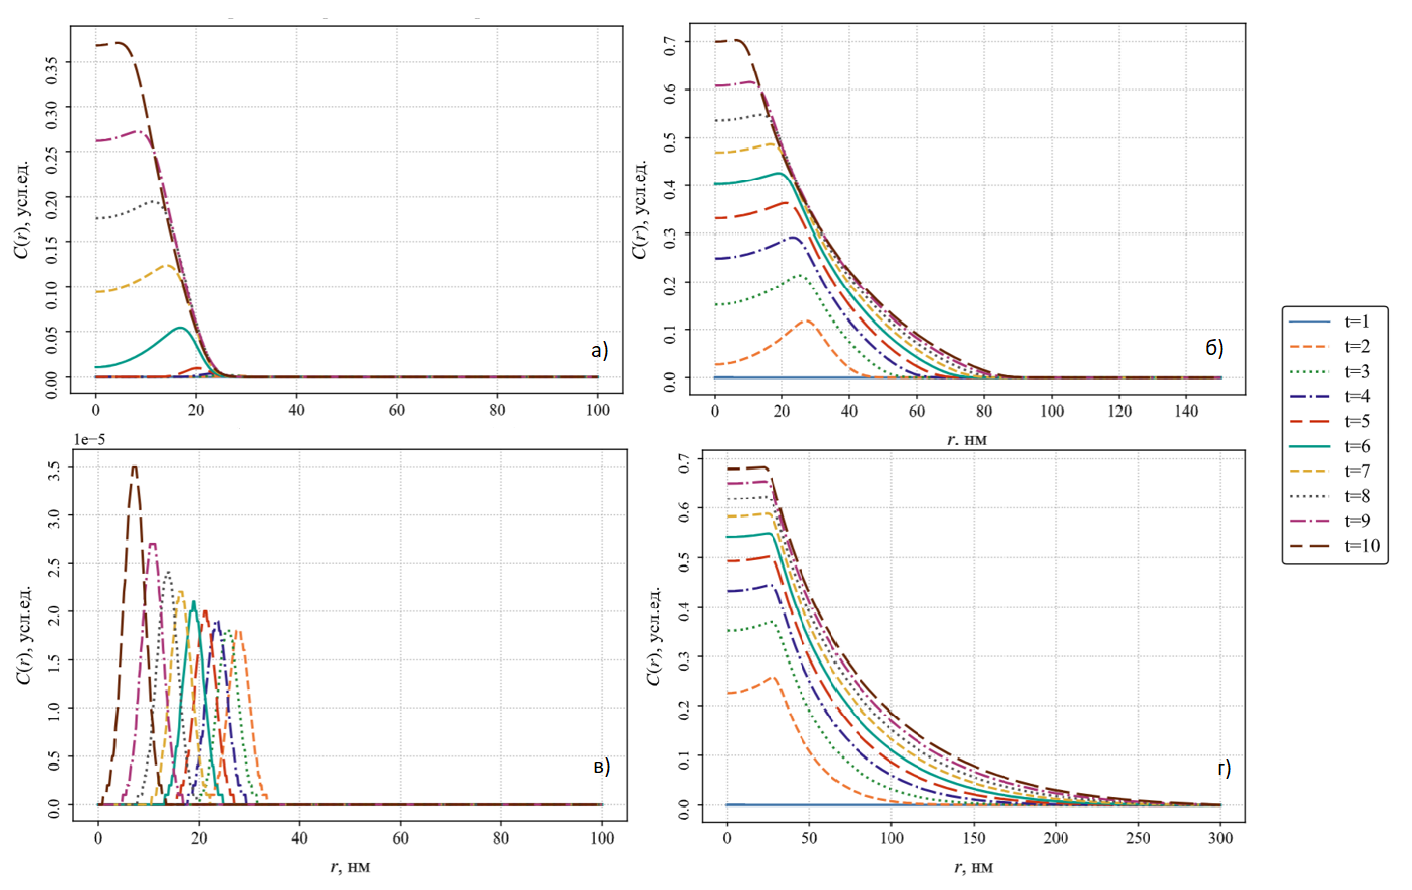
\includegraphics[width=18cm]{images/C_Ga_t.png}
    \caption{\label{fig:c_ga_t} Распределение концентрации атомов галлия $C_{\text{Ga}}(r, t)$ при разных температурах: (а)~$T = 170^\circ$C, (б)~$T = 250^\circ$C, (в)~$T = 300^\circ$C и (г)~$T = 400^\circ$C.}
    \end{center}
\end{figure}

\begin{figure}[H]
    \begin{center}
    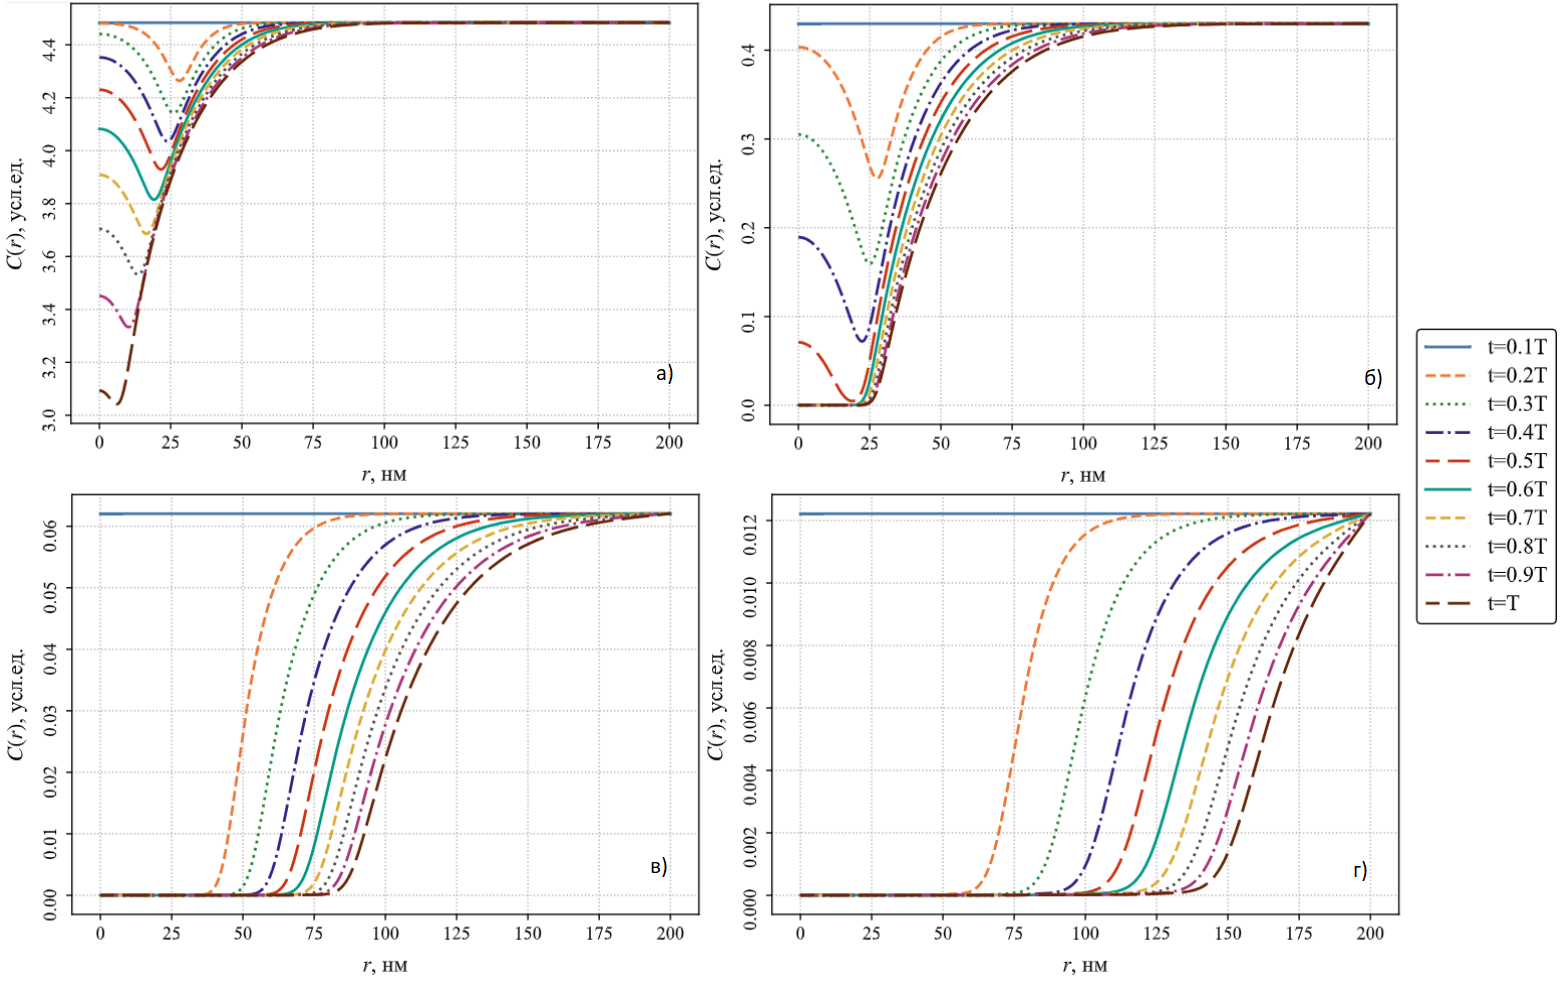
\includegraphics[width=18cm]{images/C_As_t.png}
    \caption{\label{fig:c_as_t} Распределение концентрации атомов мышьяка $C_{\text{As}}(r, t)$ при разных температурах:(а)~$T = 170^\circ$C, (б)~$T = 250^\circ$C, (в)~$T = 300^\circ$C и (г)~$T = 400^\circ$C.}
    \end{center}
\end{figure}

Для наглядности на рис.~\ref{fig:diff_length_as} представлена зависимость длины диффузии мышьяка от температуры. Видно, что при понижении температуры $L_{\mathrm{As}}$ экспоненциально возрастает, достигая сотен нанометров, тогда как при высоких температурах десорбция преобладает, и диффузия становится крайне ограниченной. Эта зависимость оказывает ключевое влияние на механизм роста и тип формируемой структуры.

\begin{figure}[H]
    \begin{center}
    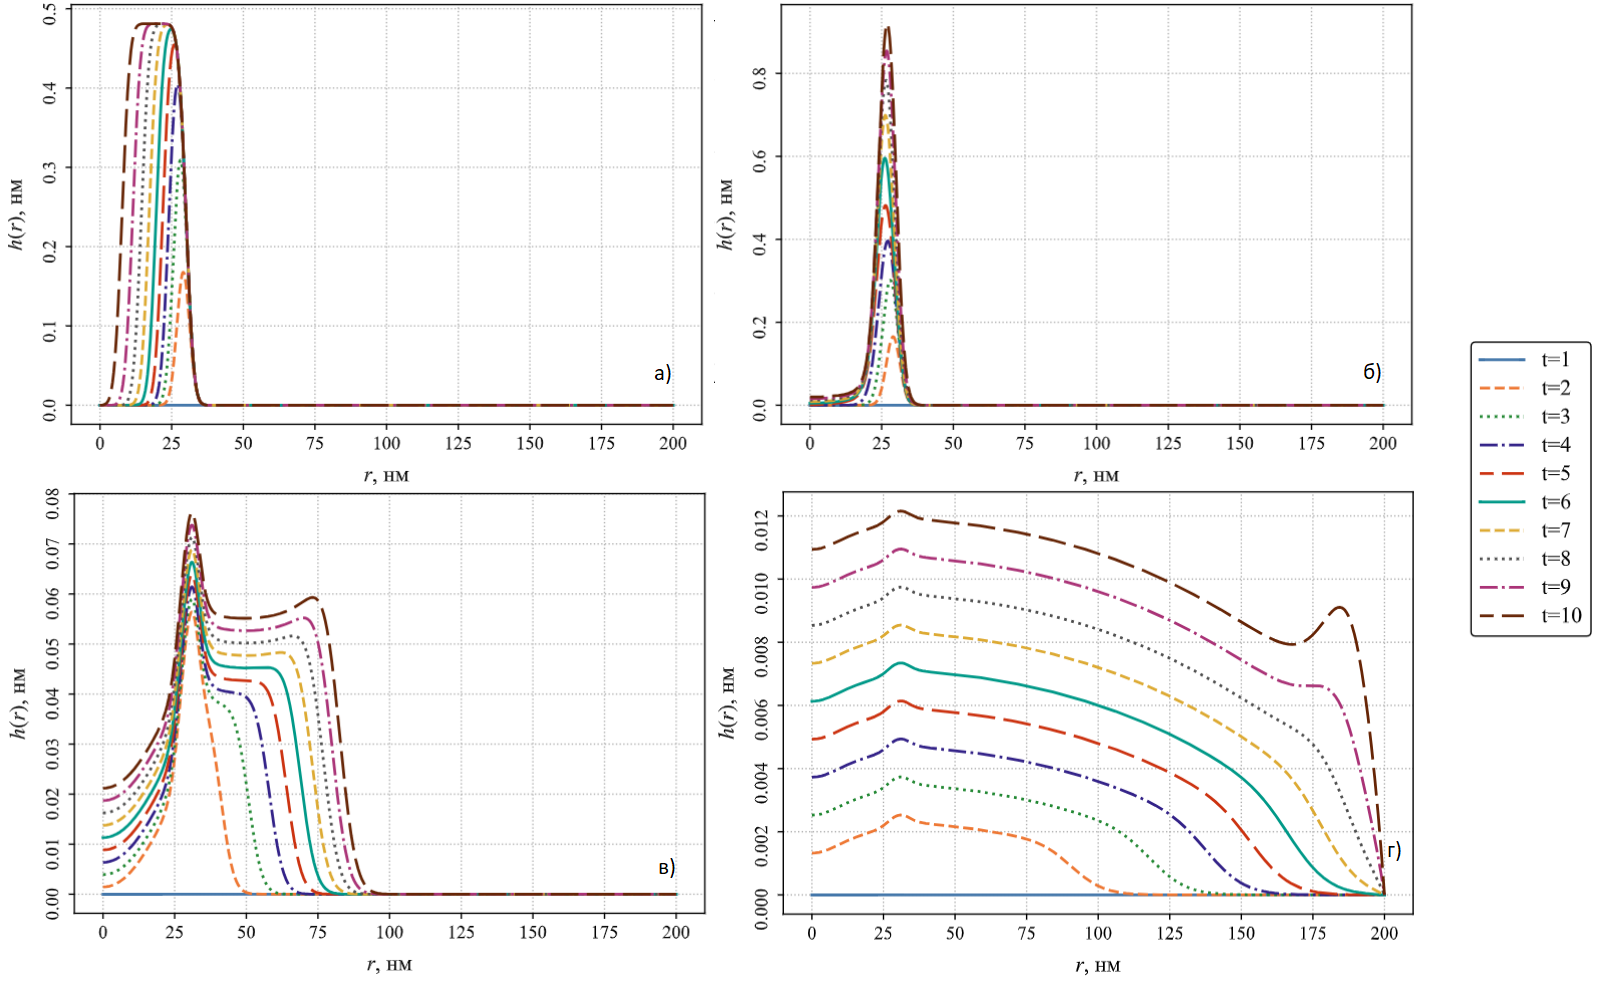
\includegraphics[width=18cm]{images/h-t.png}
    \caption{\label{fig:h_t} Профиль высоты кольца $h(r, t)$ во времени при различных температурах:(а)~$T = 170^\circ$C, (б)~$T = 250^\circ$C, (в)~$T = 300^\circ$C и (г)~$T = 400^\circ$C.}
    \end{center}
\end{figure}

\begin{figure}[H]
    \begin{center}
    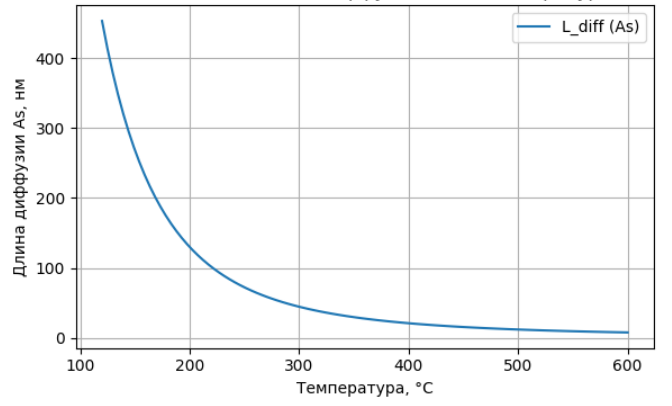
\includegraphics[width=15cm]{images/L_diff_As.png}
    \caption{\label{fig:diff_length_as} Зависимость длины диффузии атомов мышьяка от температуры.}
    \end{center}
\end{figure}
    
\textbf{Низкая температура (T = 170\textdegree C)} (рис. 4.1а, 4.2а, 4.3а) соответствует кинетически ограниченному режиму, в котором рост структуры формируется преимущественно под действием локализованного потока галлия. Длина диффузии мышьяка в этом режиме составляет 196{,}9~нм, что указывает на высокую подвижность атомов As, несмотря на низкую температуру.

График концентрации мышьяка $C_\mathrm{As}(r, t)$ (рис. 4.2а) показывает, что As активно накапливается на периферии, но его концентрация в центральной области существенно ниже~— особенно на ранних этапах. Только к поздним временам профиль становится более пологим и приближается к насыщению. Это указывает на то, что, несмотря на относительно высокую длину диффузии, распределение As по поверхности не является равномерным.

Профиль концентрации галлия $C_\mathrm{Ga}(r, t)$ (рис. 4.1а) остаётся резко локализованным. Поток $F_\mathrm{Ga}(r, t)$ сосредоточен вблизи центра ($r = 0$) и имеет узкую гауссову форму. Следовательно, реакция Ga~+~As~$\rightarrow$~GaAs происходит только в области, где оба компонента перекрываются~— в центре.

На графике высоты $h(r)$ (рис. 4.3а) широкий пик в центре, а высота быстро затухает при увеличении радиуса. Морфология структуры напоминает компактную каплю, локализованную строго вблизи $r = 0$. Такая форма характерна для систем, в которых зона перекрытия галлия и мышьяка ограничена центром из-за низкой диффузии Ga и отсутствия условий для радиального роста.

Важно отметить, что при этих условиях не формируется кольцевая структура: отсутствует центральный провал, нет периферийного вала, и вся масса материала сосредоточена в одной точке. Это позволяет интерпретировать наблюдаемую морфологию как аналог квантовой точки, формируемой в условиях капельной эпитаксии.

Подобный режим, при котором локализованный поток Ga и начальная фаза взаимодействия с As приводят к росту точечной наноструктуры, описан в теоретической модели в работе~\cite{zhou2013}. Согласно этой модели, квантовая точка формируется в случае, когда зона реакции ограничена центром капли и отсутствует эффективный радиальный перенос.

\textbf{Средняя температура (T = 250\textdegree C)} (рис. 4.1б, 4.2б, 4.3б) создаёт условия для устойчивого роста одиночного квантового кольца. Длина диффузии мышьяка составляет 72{,}33~нм, обеспечивая равномерное распределение As по поверхности подложки.

График $C_\mathrm{As}(r, t)$ (рис. 4.2б) демонстрирует, что на ранних этапах роста концентрация мышьяка в центре понижена, но затем профиль выравнивается и достигает насыщения. Галлий, напротив, остаётся локализованным вблизи центра: его концентрация $C_\mathrm{Ga}(r, t)$ (рис. 4.1б) резко падает уже при $r \approx 20$--25~нм. Таким образом, зона реакции смещается в радиальном направлении — туда, где происходит перекрытие As и Ga.

Профиль высоты $h(r)$ (рис. 4.3б) чётко демонстрирует кольцевую морфологию: центральный провал и симметричный максимум по краям. Такая форма говорит об устойчивом и однородном росте. Подобная морфология наблюдалась в экспериментах, в частности, в работе~\cite{mano2005nano}, где кольца GaAs были получены при умеренных температурах методом капельной эпитаксии.

Таким образом, температурный режим при $T = 250$\textdegree C можно считать оптимальным для формирования одиночного симметричного квантового кольца с хорошо контролируемыми параметрами.

\textbf{Переходная температура (T = 300\textdegree C)} (рис. 4.1в, 4.2в, 4.3в) соответствует началу перестройки морфологии кольца. В этом режиме зона реакции смещается на периферию, наблюдается неравномерная кристаллизация, а форма структуры становится широкой и несимметричной.

Длина диффузии мышьяка составляет 44{,}58~нм, что ниже, чем при $T = 250$\textdegree C. Как видно из графика $C_\mathrm{As}(r, t)$ (рис. 4.2в), на ранних этапах As практически отсутствует в центральной зоне и накапливается только на расстоянии порядка 70--80~нм от центра. По мере времени фронт смещается внутрь, но насыщения в центре не достигается, что ограничивает реакцию GaAs в этой области.

Профиль концентрации галлия $C_\mathrm{Ga}(r, t)$ (рис. 4.1в) демонстрирует нетипичную картину: максимум находится не в центре, а на расстоянии порядка 30--40~нм. Это связано с перераспределением вещества при уменьшении радиуса капли и, вероятно, с повышенной подвижностью поверхности.

Результатом такого смещения зон активности становится изменённый профиль высоты $h(r)$ (рис. 4.3в): центральный провал становится менее выраженным, появляется широкое плато и намечается вторичный максимум. Такая структура является переходной между одиночным и двойным кольцом.

Похожие морфологии наблюдались в экспериментах, описанных в работе~\cite{mano2005nano}, где при увеличении температуры формировались концентрические двойные кольца GaAs. Таким образом, при $T = 300$\textdegree C начинается перестройка механизма роста и появление признаков более сложной кольцевой топологии.

\textbf{Высокая температура (T = 400\textdegree C)} (рис. 4.1г, 4.2г, 4.3г) соответствует режиму, при котором рост квантовой структуры практически подавлен. Основная причина~— высокая скорость десорбции мышьяка с поверхности подложки, что делает невозможной эффективную кристаллизацию соединения GaAs.

Численно рассчитанная длина диффузии As составляет всего 21{,}01~нм — это минимальное значение среди всех температурных режимов. График концентрации мышьяка $C_\mathrm{As}(r, t)$ (рис. 4.2г) подтверждает это: в центральной области концентрация близка к нулю, заметное накопление наблюдается только на периферии. Даже по мере времени профиль остаётся обеднённым.

В то же время профиль $C_\mathrm{Ga}(r, t)$ (рис. 4.1г) сохраняет свою форму, с максимумом в центре. Галлий по-прежнему поступает из капли, но в отсутствие достаточного количества мышьяка реакция практически не протекает.

График высоты $h(r)$ (рис. 4.3г) демонстрирует крайне низкие значения — порядка 0.01~нм. Профиль размыт, нет чёткого пика или кольцевой формы. Это означает, что осаждение GaAs существенно ограничено: рост либо отсутствует, либо осуществляется на уровне фонообразного шума.

Аналогичное поведение было описано в работе~\cite{fan2023evaporation}, где рост GaAs-структур при высоких температурах ограничивался испарением As, что приводило к подавлению кристаллизации. В таких условиях вместо кольца формируется слабый, почти плоский “диск” без центрального провала.

Таким образом, при $T = 400$\textdegree C рост практически блокируется: единственный поступающий компонент — галлий — не может реализовать фазовый переход без присутствия As, который десорбируется до начала реакции.

\subsection{Анализ влияния потока мышьяка на формирование кольца}

Для оценки влияния интенсивности потока атомов мышьяка на морфологию квантового кольца была проведена серия численных экспериментов с фиксированной температурой \(T = 250^\circ C\), геометрией капли и другими параметрами модели. Варьировался лишь параметр флюкса \( F_{\text{As}} \), с тремя значениями: (а)~\(2 \times 10^{-11}\) нм$^{-2}$с$^{-1}$, (б)~\(1 \times 10^{-10}\) нм$^{-2}$с$^{-1}$ (базовый режим), (в)~\(4 \times 10^{-10}\) нм$^{-2}$с$^{-1}$.

Результаты моделирования представлены на рис.~\ref{fig:ga_flux_2}–\ref{fig:h_flux_2} и демонстрируют распределения концентраций галлия, мышьяка, а также профили высоты кольца на различных временных срезах.

\begin{figure}[H]
    \begin{center}
    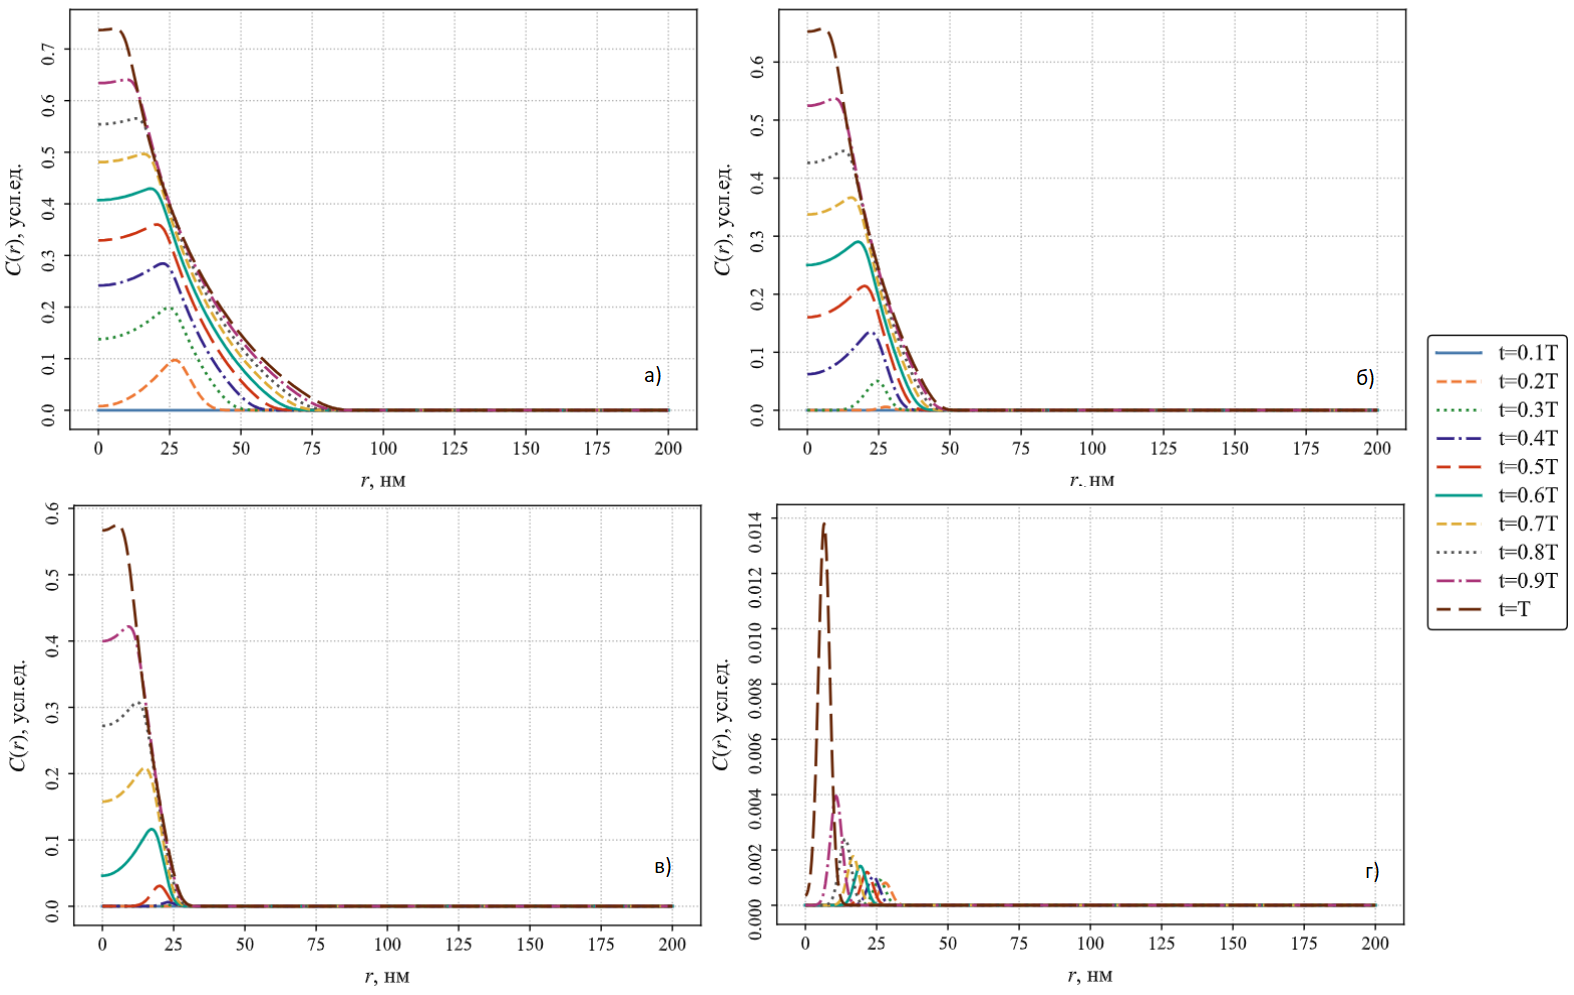
\includegraphics[width=15cm]{images/C_Ga_t_2.png}
    \caption{\label{fig:ga_flux_2} Распределение концентрации галлия $C_{\text{Ga}}(r)$ во времени при различных потоках мышьяка: (а)~$F_{\text{As}} = 2 \times 10^{-11}$ нм$^{-2}$с$^{-1}$, (б)~$1 \times 10^{-10}$ нм$^{-2}$с$^{-1}$, (в)~$4 \times 10^{-10}$ нм$^{-2}$с$^{-1}$.}
    \end{center}
\end{figure}

\begin{figure}[H]
    \begin{center}
    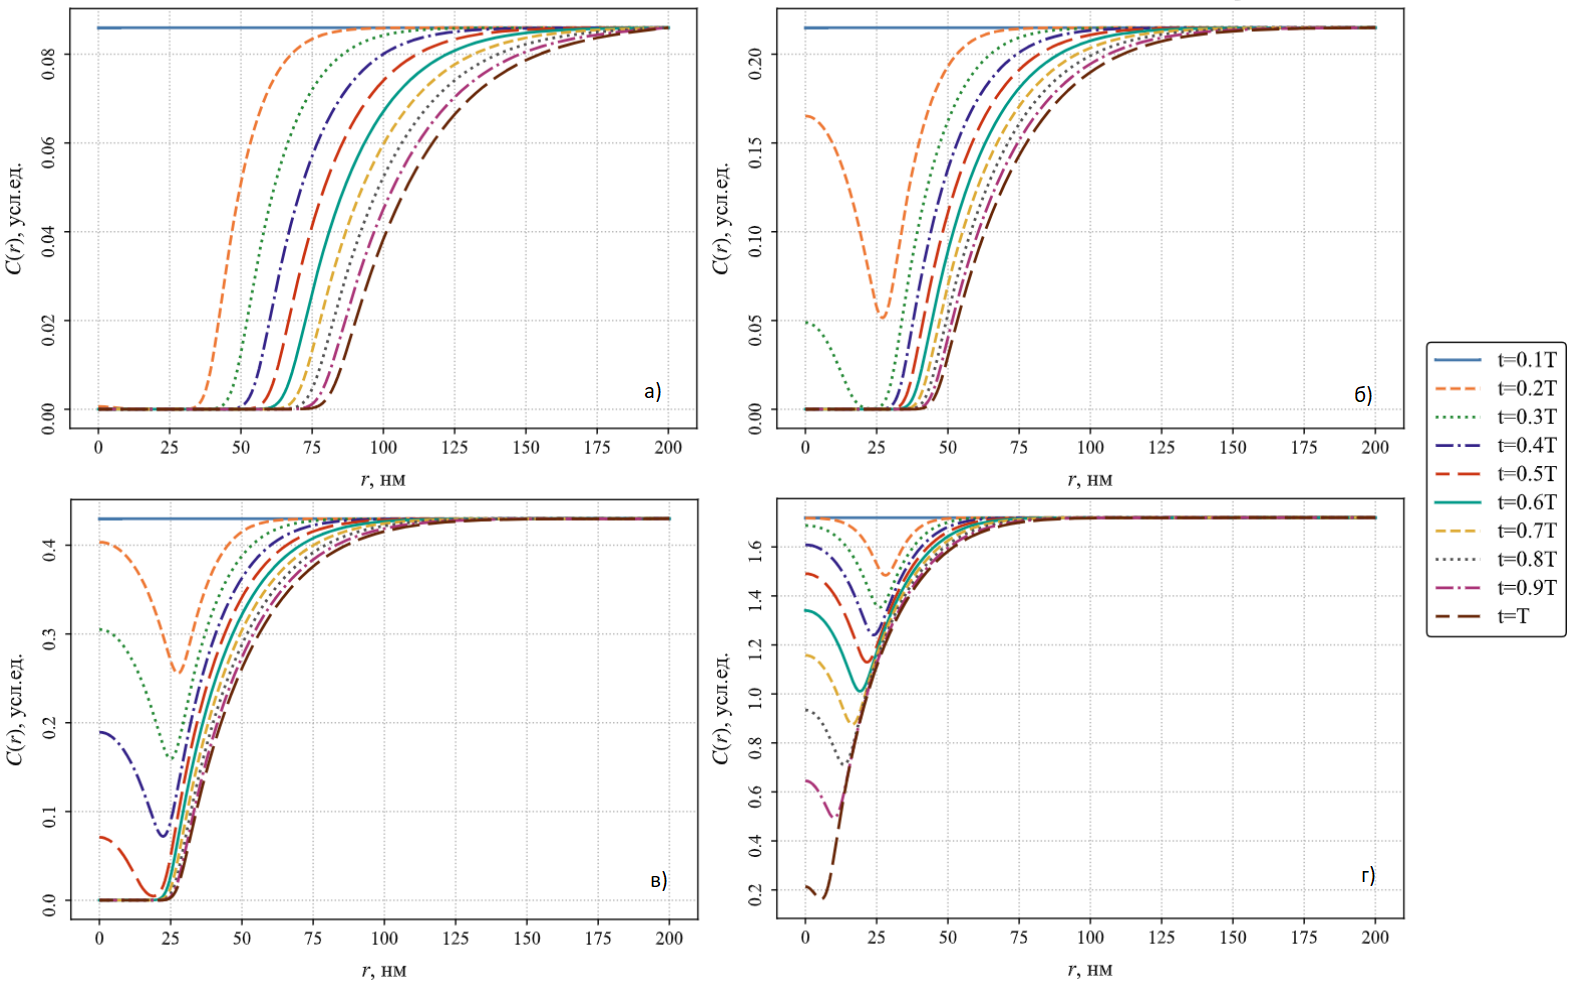
\includegraphics[width=15cm]{images/C_As_t_2.png}
    \caption{\label{fig:as_flux_2} Распределение концентрации мышьяка $C_{\text{As}}(r)$ во времени при различных потоках $F_{\text{As}}$: (а)~$2 \times 10^{-11}$, (б)~$1 \times 10^{-10}$, (в)~$4 \times 10^{-10}$ нм$^{-2}$с$^{-1}$.}
    \end{center}
\end{figure}

\begin{figure}[H]
    \begin{center}
    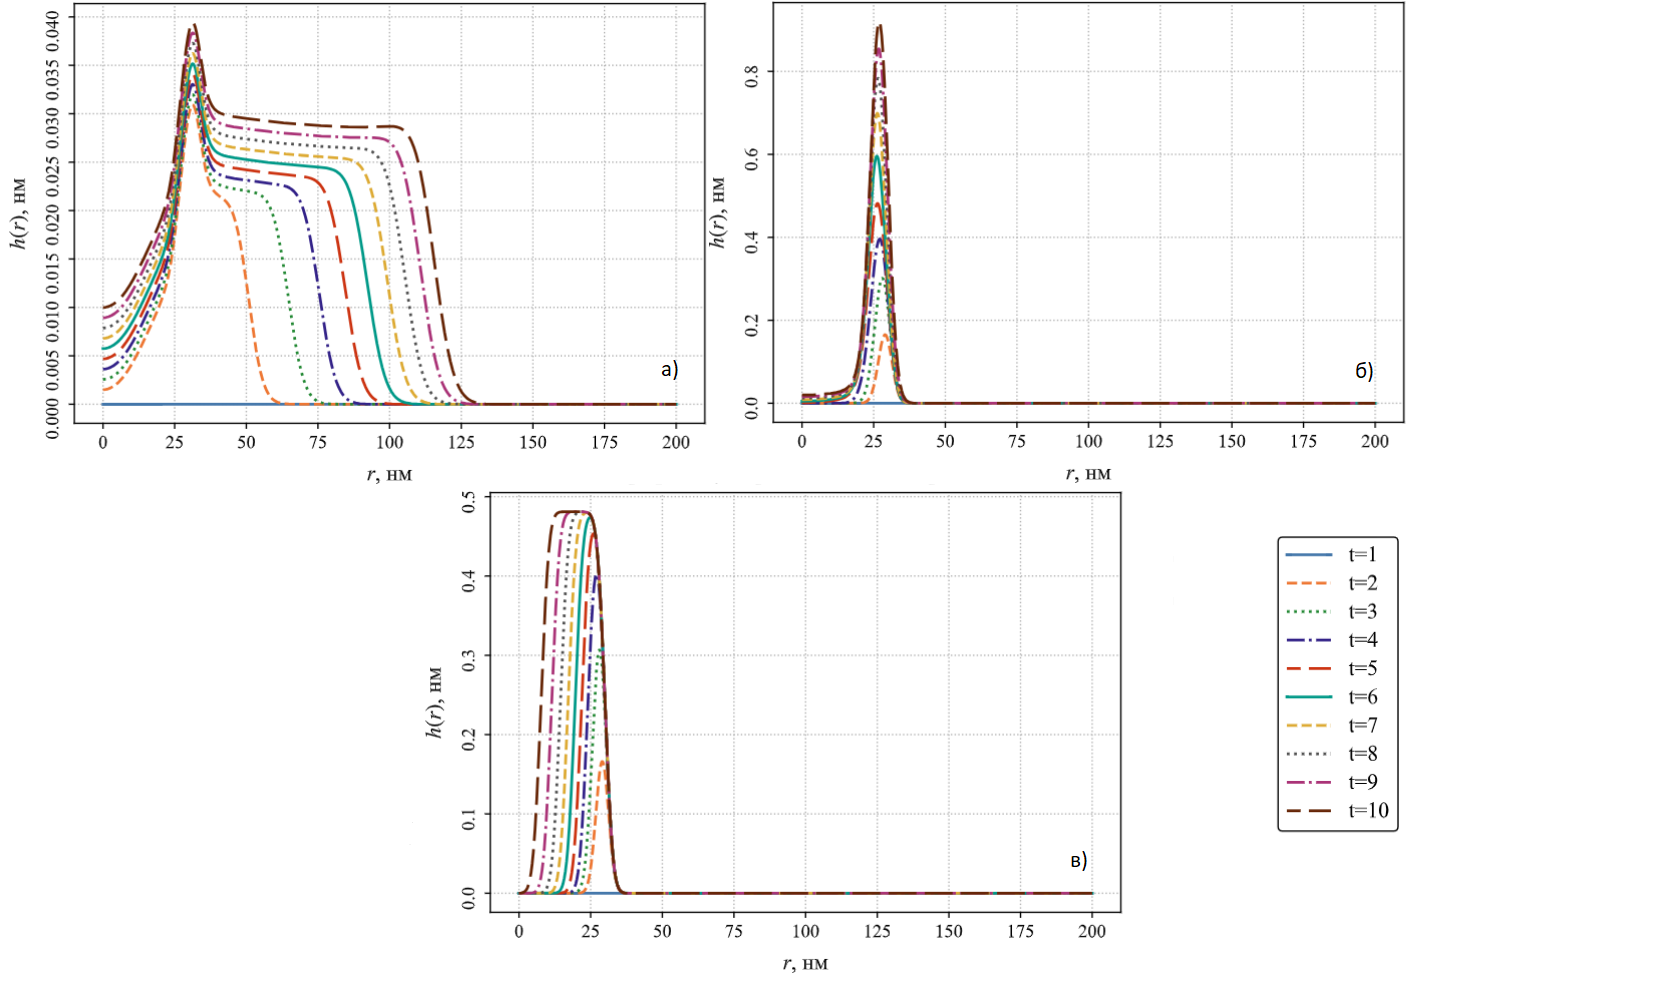
\includegraphics[width=15cm]{images/h_t_2.png}
    \caption{\label{fig:h_flux_2} Профиль высоты кольца $h(r)$ во времени при различных потоках мышьяка: (а)~$F_{\text{As}} = 2 \times 10^{-11}$, (б)~$1 \times 10^{-10}$, (в)~$4 \times 10^{-10}$ нм$^{-2}$с$^{-1}$.}
    \end{center}
\end{figure}


\textbf{Сильно пониженный поток мышьяка ($F_\mathrm{As} = 2 \times 10^{-11}~\text{нм}^{-2}\text{с}^{-1}$)} (рис. 4.5а, 4.6а, 4.7а) соответствует режиму, в котором образование GaAs-структуры практически невозможно вследствие крайней нехватки атомов мышьяка. Это экстремальное условие моделирует ситуацию, при которой поток мышьяка недостаточен для инициирования полноценной кристаллизации даже в присутствии капли галлия.

Профиль концентрации мышьяка $C_\mathrm{As}(r, t)$ (рис. 4.6а) показывает, что вещество практически не накапливается ни в центральной зоне, ни на периферии. Даже к позднему времени значения концентрации остаются близкими к нулю по всей области. Это указывает на то, что атомы As либо десорбируются сразу после осаждения, либо не достигают поверхности в достаточном количестве. Такая картина полностью согласуется с результатами моделирования, представленными в работе~\cite{fan2023evaporation}, где описан аналогичный режим с подавлением роста вследствие испарения мышьяка.

Профиль галлия $C_\mathrm{Ga}(r, t)$ (рис. 4.5а) показывает, что поток Ga, хотя и локализован вблизи центра, распространяется немного шире, чем в температурно ограниченных режимах. Однако, в отсутствие достаточного количества As, реакция Ga~+~As~$\rightarrow$~GaAs практически не происходит.

На графике высоты $h(r)$ (рис. 4.7а) это выражается в виде слабого центрального подъёма без характерной кольцевой формы. Максимальная высота структуры не превышает долей нанометра, профиль пологий, слабо выраженный, без чёткого вала. По сути, формируется не кольцо, а усреднённый куполообразный наноскопический дефект.

Таким образом, при сильно пониженном потока мышьяка ограничивающим фактором роста является именно отсутствие второго компонента. Даже в присутствии капли галлия процесс кристаллизации GaAs не реализуется, что приводит к срыву формирования квантовой структуры.

\textbf{Базовый поток мышьяка ($F_\mathrm{As} = 1 \times 10^{-10}~\text{нм}^{-2}\text{с}^{-1}$)} (рис. 4.5б, 4.6б, 4.7б). Режим при $F_\mathrm{As} = 1 \times 10^{-10}~\text{нм}^{-2}\text{с}^{-1}$ соответствует базовому сценарию, уже подробно рассмотренному в разделе~4.1 при температуре $T = 250$\textdegree C. Здесь достигается сбалансированное перекрытие компонентов Ga и As, обеспечивающее устойчивый рост одиночного кольца.
 
\textbf{Повышенный поток мышьяка ($F_\mathrm{As} = 4 \times 10^{-10}~\text{нм}^{-2}\text{с}^{-1}$)} (рис. 4.5в, 4.6в, 4.7в) приводит к заметным изменениям в морфологии кольца. При избыточном поступлении As нарушается сбалансированность между компонентами, что влияет на локализацию зоны реакции и симметрию структуры.

Профиль концентрации мышьяка $C_\mathrm{As}(r, t)$ (рис. 4.6в) демонстрирует раннее насыщение по всей поверхности, включая периферию. Мышьяк становится практически неограничивающим фактором: его присутствие в избытке обеспечивает полное покрытие подложки, но не способствует избирательному росту.

Профиль $C_\mathrm{Ga}(r, t)$ (рис. 4.5в) остаётся относительно локализованным, но начинает сдвигаться в периферийную область. Это может быть связано с перераспределением потока в условиях избытка As. В результате зона эффективного перекрытия компонентов размывается и смещается, снижая пространственную селективность роста.

На графике высоты $h(r)$ (рис. 4.7в) наблюдается более сложная форма: основной максимум становится менее симметричным, центральный провал уменьшается, и структура теряет характерный выраженный вал. Всё более выраженное сглаживание профиля и исчезновение центрального провала свидетельствуют о том, что структура топологически стремится к форме куполообразной наноструктуры — квантовой точки. Таким образом, избыток мышьяка приводит к потере радиальной избирательности роста, и структура переходит от кольцевой формы к морфологии, типичной для точечного осаждения.

Похожие эффекты описаны в работе~\cite{fan2023evaporation}, где при усилении флюкса As наблюдалась потеря симметрии, расширение зон осаждения и сглаживание структуры. Также, как показано в~\cite{mano2005nano}, отклонения от оптимального потока приводят к нарушению топологической стабильности кольца.

Таким образом, при повышенном потоке мышьяка структура теряет чёткость, и рост выходит за рамки строго контролируемого кольца, переходя либо к неустойчивому многозонному осаждению, либо к упрощённой морфологии, характерной для квантовой точки.

%  ВЫВОДЫ И ЗАКЛЮЧЕНИЕ
% ============================================
\pagebreak
\specialsection{Заключение}

В данной работе была построена и реализована численная модель капельной эпитаксии квантовых колец, описывающая пространственно-временное распределение атомов галлия и мышьяка, их взаимодействие и изменение формы капли. Модель основана на реакционно-диффузионном подходе с осевой симметрией и учитывает реалистическое распределение потока Ga с его усыханием во времени.

Проведённая серия численных экспериментов продемонстрировала, что морфология формирующихся структур критически зависит от условий роста: температуры и интенсивности потока мышьяка. Были выявлены следующие закономерности:

\begin{itemize}
    \item При низкой температуре или повышенном потоке мышьяка структура стремится к куполообразной морфологии, типичной для квантовой точки.
    \item Оптимальные условия ($T \approx 250$\textdegree C, сбалансированный поток As) обеспечивают устойчивое формирование одиночного симметричного кольца.
    \item Повышение температуры приводит к нарушению симметрии и формированию двойных или многозонных структур.
\end{itemize}

Результаты вычислений по разработанной модели качественно соответствуют известным экспериментальным данным: при увеличении температуры и уменьшении потока мышьяка радиус кольца увеличивается, а форма структуры меняется от одиночного кольца к двойному или к сплошному диску. Полученные морфологические переходы при варьировании ключевых параметров роста согласуются с теоретическими моделями и физическими механизмами, описанными в работах~\cite{zhou2013,mano2005nano,fan2023evaporation}. Это подтверждает корректность использованного подхода и его применимость для анализа и прогнозирования процессов капельной эпитаксии.

Ключевым преимуществом предложенной модели является её динамический характер: диффузия и рост описываются как функции времени, что позволяет учитывать эволюцию концентрационных профилей и морфологии в процессе роста. В отличие от большинства известных моделей, использующих стационарные приближения диффузии~\cite{zhou2013}, в данной модели решаются нестационарные уравнения, отражающие реальные кинетические процессы.

В дальнейшем перспективным направлением развития модели является учёт пространственной анизотропии коэффициента диффузии, которая может существенно повлиять на распределение мышьяка по поверхности и, как следствие, на форму формирующейся наноструктуры. Особенно важно это при моделировании процессов на кристаллических подложках с выраженной анизотропией, где диффузия вдоль различных кристаллографических направлений отличается. Кроме того, предполагается учесть эллиптическую (в общем случае неосесимметричную) форму капли, что позволит описывать более широкий класс ситуаций, включая асимметричные структуры и условия, приближенные к реальному эпитаксиальному росту.

\clearpage
\addcontentsline{toc}{section}{Список литературы}
\printbibliography


% ---приложения ---
\clearpage
\appendix

\section*{Приложение A. Код программы}
\addcontentsline{toc}{section}{Приложение A. Код программы}

\begin{lstlisting}[language=Rust]
    use indicatif::ProgressBar;

    mod file;
    
    fn main() {
        // Fixed parameters
        let a0: f64 = 0.565/2.0; // nm
        let omega_ga = a0.powi(3);     // nm^3
        let c0 = 1.0/a0.powi(2);           // nm^-2
        let e_ga = 0.5;  // eV
        let e_as: f64 = 0.5; // eV
        let e_a: f64 = 1.0;  // eV
    
        // User-defined parameters
        let temperature = 250.0; // temperature in C
        let kt = 8.62e-5*(273.0+temperature); // Temperature in eV
        let nu0 = 2e6*kt/4.136; // GHz or ns^-1
    
        let flux_relative = 0.25*1e-10; // relative flux, correct order, do not change the order
        let f_as = c0*nu0*flux_relative;         // As flux, nm^(-2)/ns
    
        let d_ga = nu0/c0*(-e_ga/kt).exp(); // diffusion coefficient
        let d_as = nu0/c0*(-e_as/kt).exp(); // nm^2 / ns
        let tau_as = (e_a / kt).exp()/nu0;
        let diff_length_as = (d_as*tau_as).sqrt(); // nm
        println!("As diffusion length is {} nm", diff_length_as);
        let kr = d_ga;           // nm^2 / ns ! just a guess, may need to change
        let w: f64 = 3.0;            // width of Gaussian flux, nm
        let r_inf = 200.0;      // domain size, nm
        let theta = 60.0;       // contact angle in degrees
        let rd_initial: f64 = 30.0; // nm
        let h0 = a0;           // cell height per layer
    
        // Derived parameters
        let theta_rad: f64 = theta / 180.0 * std::f64::consts::PI;
        let numerator_b = 8.0 - 9.0 * theta_rad.cos() + (3.0 * theta_rad).cos();
        let denominator_b = 3.0 * theta_rad.sin() - (3.0 * theta_rad).sin();
        let b_theta = numerator_b / denominator_b;
    
        // Grid setup
        let nr = 1000;
        let dr = r_inf / nr as f64;
        let dr2 = dr*dr;
        let r: Vec<f64> = (0..=nr).map(|i| i as f64 * dr).collect();
        let dt = dr2 / d_ga / 10.0;
    
        // Precompute coefficients
        let alpha = d_ga * dt / dr2;
        let beta =  d_as * dt / dr2;
        let omega = c0 * kr * dt;
        let kappa = dt * f_as / c0;
        let gamma = dt / tau_as;
        let epsilon = (f_as * tau_as) / c0;
        // See Ga flux calculation below, same as before
        let flux_factor = dt * 2.0*d_ga/w.powi(2);
        let flux_radius2 = 4.0*d_ga*c0/f_as;
        let r03_droplet_coefficient = 2.0*omega_ga*omega*c0*dr2/b_theta;
    
        // Initial time limit
        let nt_max = 1_000_000;
    
        // Progress bar
        let pb = ProgressBar::new(nt_max as u64);
    
        // Minimal allowed droplet radius
        let rd_end: f64 = dr;
    
        // PRELIMINARY CALCULATION TO FIND FINAL TIME
        
        // Initialize arrays
        //let rj: Vec<f64> = (0..=nr).map(|j| j as f64 * dr).collect();
        let mut c_ga: Vec<f64> = vec![0.0; nr + 1];
        let mut c_as = vec![(f_as * tau_as) / c0; nr + 1];
        let mut c_ga_next = c_ga.clone();
        let mut c_as_next = c_as.clone();
        let mut rd = rd_initial;
        
        let mut jt_final = nt_max;
    
        for jt in 0..nt_max {
            pb.inc(1);
    
            // Update droplet radius
            rd = update_rho(rd, r03_droplet_coefficient, &c_ga, &c_as);
    
            if rd > rd_end {
                // Update concentrations
                update_concentrations(
                    &c_ga,
                    &c_as,
                    &mut c_ga_next,
                    &mut c_as_next,
                    rd,
                    w,
                    dr,
                    alpha,
                    beta,
                    omega,
                    gamma,
                    kappa,
                    epsilon,
                    flux_factor,
                    flux_radius2,
                    r_inf,
                    nr,
                );
                c_ga.copy_from_slice(&c_ga_next);
                c_as.copy_from_slice(&c_as_next);
            } else {
                jt_final = jt;
                break;
            }
        }
    
        let nt = jt_final;
    
        pb.finish();
    
        println!("Completed first loop, nt = {}", nt);
    
        // Progress bar
        let pb = ProgressBar::new(nt as u64);
    
        // Number of snapshots
        let ns: usize = 10;
    
        // Initialize arrays again
        let mut c_ga: Vec<f64> = vec![0.0; nr + 1];
        let mut c_as = vec![(f_as * tau_as) / c0; nr + 1];
        let mut c_ga_next = c_ga.clone();
        let mut c_as_next = c_as.clone();
        let mut h = vec![0.0; nr + 1];
        let mut h_history = vec![vec![0.0; nr + 1]; ns+1];
        let mut ga_history = vec![c_ga.clone(); ns+1];
        let mut as_history = vec![c_as.clone(); ns+1];
        let mut time_history = vec![0.0; nt];
        let mut rd_history = vec![0.0; nt];
        let mut rd = rd_initial;
    
    
        let mut js = 0;
    
        for jt in 0..nt {
            pb.inc(1);
    
            // Update droplet radius
            rd = update_rho(rd, r03_droplet_coefficient, &c_ga, &c_as);
    
            // Update height profile
            for j in 0..=nr {
                h[j] += omega * h0 * c_ga[j] * c_as[j];
            }
    
            if jt % (nt / ns) == 0 {
                h_history[js] = h.clone();
                ga_history[js] = c_ga.clone();
                as_history[js] = c_as.clone();
                js += 1;
            }
    
            if rd > rd_end {
                time_history[jt] = jt as f64 * dt;
                rd_history[jt] = rd;
    
                // Update concentrations
                update_concentrations(
                    &c_ga,
                    &c_as,
                    &mut c_ga_next,
                    &mut c_as_next,
                    rd,
                    w,
                    dr,
                    alpha,
                    beta,
                    omega,
                    gamma,
                    kappa,
                    epsilon,
                    flux_factor,
                    flux_radius2,
                    r_inf,
                    nr,
                );
                c_ga.copy_from_slice(&c_ga_next);
                c_as.copy_from_slice(&c_as_next);
            } else {
                break;
            }
        }
    
        pb.finish();
        println!("Completed second loop, now saving files!");
    
        h_history.push(r.clone());
        ga_history.push(r.clone());
        as_history.push(r);
    
        file::save_columns_to_file(&vec![time_history, rd_history], "results", "droplet.dat");
        file::save_columns_to_file(&h_history, "results", "height.dat");
        file::save_columns_to_file(&ga_history, "results", "c_ga.dat");
        file::save_columns_to_file(&as_history, "results", "c_as.dat");
    
    }
    
    fn update_concentrations(
        c_ga: &[f64],
        c_as: &[f64],
        c_ga_next: &mut [f64],
        c_as_next: &mut [f64],
        rd: f64,
        w: f64,
        dr: f64,
        alpha: f64,
        beta: f64,
        omega: f64,
        gamma: f64,
        kappa: f64,
        epsilon: f64,
        flux_factor: f64,
        flux_radius2: f64,
        r_inf: f64,
        nr: usize,
    ) {
    
        // Handle j=0
        // Ga flux calculation using the formulas, derived before, now gives a correct result
        c_ga_next[0] = c_ga[0] + 4.0 * alpha * (c_ga[1] - c_ga[0])
            - omega * c_ga[0] * c_as[0]
            + flux_factor * wp_j(0.0, rd, w)
            / (3.545 * rd / w + 0.187 * w / (r_inf - 3.156 * w))
            / (r_inf / rd).ln();
        c_as_next[0] = c_as[0] + 4.0 * beta * (c_as[1] - c_as[0]) 
            - gamma * c_as[0] 
            + kappa 
            - omega * c_ga[0] * c_as[0];
    
        // Handle interior points
        for j in 1..nr {
            let j_f64 = j as f64;
            let coeff = 1.0 / (2.0 * j_f64);
            
            // gallium atoms
            let term_ga = alpha * (
                (1.0 + coeff) * c_ga[j + 1] 
                - 2.0 * c_ga[j] 
                + (1.0 - coeff) * c_ga[j - 1]
            );
            // Ga flux calculation 3rd version from the notes
            let conc_ratio = flux_radius2/rd.powi(2);
            let rd_rinf_ratio2 = r_inf.powi(2)/rd.powi(2);
            let additional_factor = 1.0 + (rd_rinf_ratio2 - 1.0 + rd_rinf_ratio2.ln())/conc_ratio;
            c_ga_next[j] = c_ga[j] + term_ga
            - omega * c_ga[j] * c_as[j]
            + flux_factor * additional_factor * wp_j(j_f64 * dr, rd, w)
            / (3.545 * rd / w + 0.187 * w / (r_inf - 3.156 * w))
            / (r_inf / rd).ln();
            // as atoms
            let term_as = beta * (
                (1.0 + coeff) * c_as[j + 1] 
                - 2.0 * c_as[j] 
                + (1.0 - coeff) * c_as[j - 1]
            );
            c_as_next[j] = c_as[j] + term_as - gamma * c_as[j] + kappa 
                - omega * c_ga[j] * c_as[j];
        }
    
        // Boundary conditions
        c_ga_next[nr] = 0.0;
        c_as_next[nr] = epsilon;
    }
    
    fn update_rho(rd: f64, r03: f64, c_ga: &[f64], c_as: &[f64]) -> f64 {
        let sum = multiply_sum_with_index(c_ga, c_as);
        rd - r03/rd*sum
    }
    
    fn multiply_sum_with_index(a: &[f64], b: &[f64]) -> f64 {
        assert_eq!(a.len(), b.len(), "Arrays must have the same length");
        a.iter()
            .zip(b.iter())
            .enumerate()
            .map(|(i, (&a_val, &b_val))| a_val * b_val * i as f64)
            .sum()
    }
    
    fn wp_j(x: f64, x0: f64, w: f64) -> f64 {
        let x2 = -((x-x0)/w).powi(2);
        x2.exp()
    } 
\end{lstlisting}

\end{document}
